\documentclass[a4paper,fleqn,usenatbib]{mnras}

\usepackage{ae, aecompl, amsmath, amssymb}
\usepackage{bm}           %%  bold math
\usepackage{cancel, mathptmx}
\usepackage{color}
\usepackage{dcolumn}  %%  Align table columns on decimal point
\usepackage{epsfig, epsf, etoolbox}
\usepackage{fancyhdr}
\usepackage{graphicx}
\usepackage[T1]{fontenc}
%\usepackage{lscape}
\usepackage{ifthen}
\usepackage{hyperref}
\usepackage{listings}
\usepackage{longtable}
\usepackage{multirow}
\usepackage{newtxtext, newtxmath}
\usepackage{pifont}% http://ctan.org/pkg/pifont
\usepackage{subfigure}
\usepackage{tabu}

\usepackage{verbatim}

\usepackage{xcolor}
%\usepackage[square, sort, comma, numbers]{natbib}
\usepackage{threeparttable}
%\usepackage[square,sort,comma,numbers]{natbib}

\usepackage{graphicx}	% Including figure files
\usepackage{tikz}
\def\checkmark{\tikz\fill[scale=0.4](0,.35) -- (.25,0) -- (1,.7) -- (.25,.15) -- cycle;} 

%%  I dont know why, but arydshln leads to pdflatex crashing (when using 'regular' hline)
%% if you load this package at the top of this list.  e.g. 
%%    tex.stackexchange.com/questions/419497/hline-doesnt-compile-arydshln-and-tabularx-incompatibility
\usepackage{arydshln}


%%%%%%%%%%%%%%%%%%%%%%%%%%%%%%%%%%%%%%%%%%%
%       define Journal abbreviations      %
%%%%%%%%%%%%%%%%%%%%%%%%%%%%%%%%%%%%%%%%%%%
\def\nat{Nat} \def\apjl{ApJ~Lett.} \def\apj{ApJ}
\def\apjs{ApJS} \def\aj{AJ} \def\mnras{MNRAS}
\def\prd{Phys.~Rev.~D} \def\prl{Phys.~Rev.~Lett.}
\def\plb{Phys.~Lett.~B} \def\jhep{JHEP}
\def\npbps{NUC.~Phys.~B~Proc.~Suppl.} \def\prep{Phys.~Rep.}
\def\pasp{PASP} \def\aap{Astron.~\&~Astrophys.} \def\araa{ARA\&A}
\def\jcap{\ref@jnl{J. Cosmology Astropart. Phys.}} 
\def\nar{New~A.R.} 

\newcommand{\preep}[1]{{\tt #1} }

%%%%%%%%%%%%%%%%%%%%%%%%%%%%%%%%%%%%%%%%%%%%%%%%%%%%%
%              define symbols                       %
%%%%%%%%%%%%%%%%%%%%%%%%%%%%%%%%%%%%%%%%%%%%%%%%%%%%%
\def \Mpc {~{\rm Mpc} }
\def \Om {\Omega_0}
\def \Omb {\Omega_{\rm b}}
\def \Omcdm {\Omega_{\rm CDM}}
\def \Omlam {\Omega_{\Lambda}}
\def \Omm {\Omega_{\rm m}}
\def \ho {H_0}
\def \qo {q_0}
\def \lo {\lambda_0}
\def \kms {{\rm ~km~s}^{-1}}
\def \kmsmpc {{\rm ~km~s}^{-1}~{\rm Mpc}^{-1}}
\def \hmpc{~\;h^{-1}~{\rm Mpc}} 
\def \hkpc{\;h^{-1}{\rm kpc}} 
\def \hmpcb{h^{-1}{\rm Mpc}}
\def \dif {{\rm d}}
\def \mlim {m_{\rm l}}
\def \bj {b_{\rm J}}
\def \mb {M_{\rm b_{\rm J}}}
\def \mg {M_{\rm g}}
\def \mi {M_{\rm i}}
\def \qso {_{\rm QSO}}
\def \lrg {_{\rm LRG}}
\def \gal {_{\rm gal}}
\def \xibar {\bar{\xi}}
\def \xis{\xi(s)}
\def \xisp{\xi(\sigma, \pi)}
\def \Xisig{\Xi(\sigma)}
\def \xir{\xi(r)}
\def \max {_{\rm max}}
\def \gsim { \lower .75ex \hbox{$\sim$} \llap{\raise .27ex \hbox{$>$}} }
\def \lsim { \lower .75ex \hbox{$\sim$} \llap{\raise .27ex \hbox{$<$}} }
\def \deg {^{\circ}}
%\def \sqdeg {\rm deg^{-2}}
\def \deltac {\delta_{\rm c}}
\def \mmin {M_{\rm min}}
\def \mbh  {M_{\rm BH}}
\def \mdh  {M_{\rm DH}}
\def \msun {M_{\odot}}
\def \z {_{\rm z}}
\def \edd {_{\rm Edd}}
\def \lin {_{\rm lin}}
\def \nonlin {_{\rm non-lin}}
\def \wrms {\langle w_{\rm z}^2\rangle^{1/2}}
\def \dc {\delta_{\rm c}}
\def \wp {w_{p}(\sigma)}
\def \PwrSp {\mathcal{P}(k)}
\def \DelSq {$\Delta^{2}(k)$}
\def \WMAP {{\it WMAP \,}}
\def \cobe {{\it COBE }}
\def \COBE {{\it COBE \;}}
\def \HST  {{\it HST \,\,}}
\def \Spitzer  {{\it Spitzer \,}}
\def \ATLAS {VST-AA$\Omega$ {\it ATLAS} }
\def \BEST   {{\tt best} }
\def \TARGET {{\tt target} }
\def \TQSO   {{\tt TARGET\_QSO}}
\def \HIZ    {{\tt TARGET\_HIZ}}
\def \FIRST  {{\tt TARGET\_FIRST}}
\def \zc {z_{\rm c}}
\def \zcz {z_{\rm c,0}}


\newcommand{\sqdeg}{deg$^{-2}$}
\newcommand{\lya}{Ly$\alpha$\ }
%\newcommand{\lya}{Ly\,$\alpha$\ }
\newcommand{\lyaf}{Ly\,$\alpha$\ forest}
%\newcommand{\eg}{e.g.~}
%\newcommand{\etal}{et~al.~}
\newcommand{\cii}{C\,{\sc ii}\ }
\newcommand{\ciii}{C\,{\sc iii}]\ }
\newcommand{\civ}{C\,{\sc iv}}
\newcommand{\siiv}{Si\,{\sc iv}\ }
\newcommand{\mgii}{Mg\,{\sc ii}\ }
\newcommand{\feii}{Fe\,{\sc ii}\ }
\newcommand{\feiii}{Fe\,{\sc iii}\ }
\newcommand{\caii}{Ca\,{\sc ii}\ }
\newcommand{\halpha}{H\,$\alpha$\ }
\newcommand{\hbeta}{H\,$\beta$\ }
\newcommand{\oi}{[O\,{\sc i}]\ }
\newcommand{\oii}{[O\,{\sc ii}]\ }
\newcommand{\oiii}{[O\,{\sc iii}]\ }
\newcommand{\heii}{[He\,{\sc ii}]\ }
\newcommand{\nii}{N\,{\sc ii}\ }
\newcommand{\nv}{N\,{\sc v}\ }

%% From:: /cos_pc19a_npr/LaTeX/proposals/JWST/JWST_ERS/Proposal/lines.tex
%%  
\newcommand{\imw}{$i$--$W3$}
\newcommand{\imwf}{$i$--$W4$}
\newcommand{\rmwf}{$r$--$W4$}
\newcommand{\imwt}{$i$--$W2$}
\newcommand{\wtmwf}{$W3$--$W4$}
%\newcommand{\kms}{km s$^{-1}$}
\newcommand{\cmN}{cm$^{-2}$}
\newcommand{\cmn}{cm$^{-3}$}
%\newcommand{\msun}{M$_{\odot}$}
\newcommand{\lsun}{L$_{\odot}$}
\newcommand{\lam}{$\lambda$}
\newcommand{\mum}{$\mu$m}
\newcommand{\ebv}{$E(B$$-$$V)$}
%\newcommand{\heii}{\mbox{He\,{\sc ii}}}
\newcommand{\cv}{\mbox{C\,{\sc v}}}
%\newcommand{\civ}{\mbox{C\,{\sc iv}}}
%\newcommand{\ciii}{\mbox{C\,{\sc iii}}}
%\newcommand{\cii}{\mbox{C\,{\sc ii}}}
%\newcommand{\nv}{\mbox{N\,{\sc v}}}
\newcommand{\niv}{\mbox{N\,{\sc iv}}}
\newcommand{\niii}{\mbox{N\,{\sc iii}}}
%\newcommand{\oi}{\mbox{O\,{\sc i}}}
%\newcommand{\oii}{\mbox{O\,{\sc ii}}}
%\newcommand{\oiii}{\mbox{[O\,{\sc iii}]}}
\newcommand{\oiv}{\mbox{O\,{\sc iv}}}
\newcommand{\ov}{\mbox{O\,{\sc v}}}
\newcommand{\ovi}{\mbox{O\,{\sc vi}}}
\newcommand{\ovii}{\mbox{O\,{\sc vii}}}

%\newcommand{\feii}{\mbox{Fe\,{\sc ii}}}
%\newcommand{\feiii}{\mbox{Fe\,{\sc iii}}}
%\newcommand{\mgii}{\mbox{Mg\,{\sc ii}}}
\newcommand{\neii}{[Ne\,{\sc ii}]\ }
\newcommand{\neiii}{[Ne\,{\sc ii}]\ }
\newcommand{\nev}{Ne\,{\sc v}\ }
\newcommand{\nevi}{[Ne\,{\sc vi}]\ }
\newcommand{\neviii}{\mbox{Ne\,{\sc viii}}}
\newcommand{\aliii}{\mbox{Al\,{\sc iii}}}
\newcommand{\siii}{\mbox{Si\,{\sc ii}}}
\newcommand{\siiii}{\mbox{Si\,{\sc iii}}}
%\newcommand{\siiv}{\mbox{Si\,{\sc iv}}}
%\newcommand{\lya}{\mbox{Ly$\alpha$}}
%\newcommand{\lyb}{\mbox{Ly$\beta$}}
\newcommand{\hi}{\mbox{H\,{\sc i}}}
\newcommand{\snine}{\mbox{[S\,{\sc ix}]}}
\newcommand{\sivi}{\mbox{[Si\,{\sc vi}]}}
\newcommand{\sivii}{\mbox[{Si\,{\sc vii}]}}
\newcommand{\siix}{\mbox{[Si\,{\sc ix}]}}
\newcommand{\six}{\mbox{[Si\,{\sc x}]}}
\newcommand{\sixi}{\mbox{[Si\,{\sc xi}]}}
\newcommand{\caviii}{\mbox{[Ca\,{\sc viii}]}}
\newcommand{\arii}{\mbox{[Ar\,{\sc ii}]}}

%%[Ar II] 6.97
%% [S IX] 1.252 μm 328 
% [Si X] 1.430 μm 351 
% [Si XI] 1.932 μm 401 
% [Si VI] 1.962 μm 167 
% [Ca VIII] 2.321 μm 128 
% [Si VII] 2.483 μm 205 
% [Si IX] 3.935 μm 303
% [Ar II] 6.97


%\snine\ at 1.252$\mu$m, \six\ at 1.430$\mu$m, \sixi\ at 1.932$\mu$m, \sivi\ at
%1.962$\mu$m, \caviii\ at 2.321$\mu$m, \sivi\ at 2.483$\mu$m \siix\ at
%3.935$\mu$m and \arii\ at 6.97$\mu$m. 
%%
%% such as [Ne ii]12.8 μm, [Ne v]14.3 μm, [Ne iii]15.5 μm, [S iii]18.7 μm and 33.48 μm, [O iv]25.89 μm and [Si ii]34.8 μm (e.g
%%
%% MIR emission lines like [NeII] and [NeV] are ..
%%
%% Also,  arXiv:astro-ph/0003457v1 
%% [NeV] 14.32um & 24.32um and [NeVI] 7.65um imply an A(V)>160 towards the NLR...
%% [NeIII]15.56um/[NeII]12.81um
%%
%% [Ne V] 14.3, 24.2 μm 97.
%% [Ne II] 12.8 μm
%% [OIV] 26μm
%%


%%%%%%%%%%%%%%%%%%%%%%%%%%%%%%%%%%%%%%%%%%%%%%%%%%%%%
%              define Listings                       %
%%%%%%%%%%%%%%%%%%%%%%%%%%%%%%%%%%%%%%%%%%%%%%%%%%%%%
\definecolor{dkgreen}{rgb}{0,0.6,0}
\definecolor{gray}{rgb}{0.5,0.5,0.5}
\definecolor{mauve}{rgb}{0.58,0,0.82}

\lstset{frame=tb,
  language=Python,
  aboveskip=3mm,
  belowskip=3mm,
  showstringspaces=false,
  columns=flexible,
  basicstyle={\small\ttfamily},
  numbers=none,
  numberstyle=\tiny\color{gray},
  keywordstyle=\color{blue},
  commentstyle=\color{dkgreen},
  stringstyle=\color{mauve},
  breaklines=true,
  breakatwhitespace=true,
  tabsize=3
}

\title[High-redshift CLQs]{The first high-redshift Changing Look Quasars}

\author[Ross {\it et al.}]
{%The RH John~S.~Bercow, MP, {\it et al.} 
Nicholas~P.~Ross$^{1}$\thanks{E-mail: npross@roe.ac.uk},
 Matthew Graham$^{2}$, K. E. Saavik Ford$^{3,4,5}$,  Barry McKernan$^{3,4,5}$   
\newauthor Daniel Stern$^{6}$ and Giorgio Calderone$^{7}$
\\
% List of institutions
%$^{1}$Speaker's Chair, The House of Commons, London, SW1A 0AA \\
$^{1}$Institute for Astronomy, University of Edinburgh, Royal Observatory, Blackford Hill, Edinburgh EH9 3HJ, United Kingdom \\
$^{2}$Cahill Center for Astronomy and Astrophysics, California Institute of Technology, Mail Code 249/17, 1200 E California Blvd, Pasadena CA 91125, USA\\
$^{3}$Department of Science, BMCC, City University of New York, New York, NY 10007, USA \\
$^{4}$Department of Astrophysics, Rose Center for Earth and Space, American Museum of Natural History, Central Park West at 79th Street, NY 10024, USA \\
$^{5}$Graduate Center, City University of New York, 365 5th Avenue, New York, NY 10016, USA\\
$^{6}$Jet Propulsion Laboratory, California Institute of Technology, 4800 Oak Grove Drive, Mail Stop 169-221, Pasadena, CA 91109, USA \\
$^{7}$INAF -- Osservatorio Astronomico di Trieste, Via Tiepolo 11, I-34143 Trieste, Italy \\
}

\date{Accepted XXX. Received YYY; in original form ZZZ}
\pubyear{2018}

\hypersetup{draft}

\begin{document}
\label{firstpage}
\pagerange{\pageref{firstpage}--\pageref{lastpage}}
\maketitle

\begin{abstract}
We report on three redshift $z>2$ quasars with dramatic changes in
their \civ\ emission lines, the first ``Changing-Look'' quasars at high
redshift.  This is also the first time the changing-look behaviour has
been seen in a high-ionization emission line.
%%
SDSS J1205+3422, J1638+2827 and J2228+2201 show interesting behaviour
in their observed optical light curves, and subsequent spectroscopy
shows significant changes in the \civ\ broad emission line, with both
line collapse and emergence being displayed in rest-frame timescales
of $\sim$240-1640 days.
%%
Where observed, the profile of the Ly$\alpha$/\nv emission complex
also changes, and there is tentative evidence for changes in the \mgii
line.
%%
Although line measurements from the three quasars show large changes
in the \civ\ flux-line width plane, the quasars are not seen to
be outliers when considered against the full $z\sim2$ quasar population
in terms of (rest) Equivalent Width and FWHM properties.
%%
We put these observations in context with recent ``state-change''
models, but note that even in their `low-state', the \civ\ CLQs are
above $\sim$10\% in Eddington luminosity.
\end{abstract}



% Select between one and six entries from the list of approved keywords.
% Don't make up new ones.
\begin{keywords}
accretion, accretion discs -- surveys -- quasars: general -- quasars: individual: J1100-0053 
\end{keywords}



%%%%%%%%%%%%%%%%%%%%%%%%%%%%%%%%%%%%%%%%%%%%%%%%%%%%%%%%%%%%%%%%%%%%%%%%%%%%%%%%%
%%%%%%%%%%%%%%%%%%%%%%%%%%%%%%%%%%%%%%%%%%%%%%%%%%%%%%%%%%%%%%%%%%%%%%%%%%%%%%%%%
%%
%%
%%   SECTION 1  SECTION 1  SECTION 1  SECTION 1  SECTION 1  SECTION 1  
%%   SECTION 1  SECTION 1  SECTION 1  SECTION 1  SECTION 1  SECTION 1  
%%   SECTION 1  SECTION 1  SECTION 1  SECTION 1  SECTION 1  SECTION 1  
%%
%%
%%%%%%%%%%%%%%%%%%%%%%%%%%%%%%%%%%%%%%%%%%%%%%%%%%%%%%%%%%%%%%%%%%%%%%%%%%%%%%%%%%
%%%%%%%%%%%%%%%%%%%%%%%%%%%%%%%%%%%%%%%%%%%%%%%%%%%%%%%%%%%%%%%%%%%%%%%%%%%%%%%%%%
\section{Introduction}
Luminous AGN, i.e. quasars, are now seen to significantly vary their
energy output on timescales as short as weeks to months.  This
observation, and the subsequent mismatch in the expected ``viscous''
timescale, which for a 10$^{7}$ M$_{\odot}$ central supermassive black
hole (SMBH) is $\sim$hundreds of years, was noted over 30 years ago
\citep[e.g.][]{Alloin1985}. However, with new photometric light-curve
and repeat spectroscopic data, the desire for a deeper understanding
of AGN accretion disk physics has recently re-invigorated the field
\citep[e.g.][]{Antonucci2018, Lawrence2018, Ross2018, Stern2018}.

The optical continuum variability of quasars has been recognized since
their first optical identification
\citep[e.g.,][]{MatthewsSandage1963, MacLeod2012}.  Dramatic changes
in the broad emission lines (BELs) of quasars has only recently been
identified \citep[e.g., ][]{LaMassa2015}.  Samples of over 100
``Changing Look'' quasars (CLQs) or ``Changing State'' quasars (CSQs)
have now been assembled \citep[e.g.][]{MacLeod2019, Graham2019b}. The
community uses both these terms as a cover for the underlying
physics. For sake of argument, CLQs can potentially be thought of as
the extension to the BELs of quasar continuum variability \citep[e.g.,
][]{MacLeod2012} whereas the CSQs have a `state-transition' similar to
that in Galactic X-ray binaries \citep[][]{NodaDone2018, Ruan2019}. In
this paper, we use the term `Changing Look', as we are currently
agnostic, and confessedly ignorant, to the underlying physical
processes.

\begin{table*}
  \begin{centering}
    \begin{tabular}{l r  r r   lll lll  r r}
      \hline  \hline 
      Line                 & $\lambda$ &  Transition  & Ionization   &  \multicolumn{6}{c}{Transition Levels}                                                                                           & Wavenumber   & $A_{i,j}$                    \\
%                              &    / \AA\    &      / eV             &  / eV            &   Lower                  & Conf.      &  $J$       & Upper                      &  Conf.                       & $J$       & / cm$^{-1}$    &  / s$^{-1}$                \\      \hline
                              &  / \AA\    & energy / eV &  energy / eV  &    \multicolumn{3}{l}{Lower}    &  \multicolumn{3}{l}{Upper}                                                         & / cm$^{-1}$    & ($\times10^{8}$  / s$^{-1}$)               \\      \hline
      H LyLim           &   912.324   & 13.5984    & 13.5984        & 1$s$                    & $^2$S     & 1/2          & $\infty$                  &                                 &             & 109 678.7       & 1.23$\times10^{-6}$  \\
      H Ly$\alpha$  &  1215.670  & 10.1988    & 13.5984       & 1$s$                     & $^2$S      & 1/2          & 2                             &                                 &             &  82 259.2       &  4.67  \\
      \nv                  &  1238.821  & 10.0082    &  97.8901      &  1$s^{2}$2$s$      &  $^{2}$S   &  1/2         & 1$s^{2}$2$p$          &  $^{2}$P$^{{\rm o}}$ &   3/2    &  80 721.9        & 3.40   \\
      \nv                  &  1242.804  &  9.9762     &  97.8901      &  1$s^{2}$2$s$       &  $^{2}$S   &  1/2        &  1$s^{2}$2$p$         &  $^{2}$P$^{{\rm o}}$ &  1/2     &  80 463.2        & 3.37 \\
      \civ                 &  1548.187  &  8.0083     &  64.4935      &  1$s^{2}$2$s$       &   $^{2}$S  & 1/2         & 1$s^{2}$2$p$          &  $^{2}$P$^{{\rm o}}$ &  3/2     &  64 591.7        & 2.65  \\
      \civ                 &  1550.772  &  7.9950     &  64.4935      & 1$s^{2}$2$s$        &  $^{2}$S   & 1/2         & 1$s^{2}$2$p$          &  $^{2}$P$^{{\rm o}}$ &  1/2     &   64 484.0       & 2.64  \\
      \heii               &   1640.474  &  7.5578     & 54.4178       & 2$p$ 	      &  $^{2}$P$^{{\rm o}}$ &  3/2  &  3$d$ 	                 & $^2$D                  &  5/2        &  60 958.0       & 10.35 \\
      \heii               &   1640.490  &  7.5578     & 54.4178       & 2$p$ 	      &  $^{2}$P$^{{\rm o}}$ &  3/2  &  3$d$ 	                 & $^2$D                  &  3/2        &  60 957.4       & 1.73 \\
      \ciii                 &  1906.683  &  6.5026     & 47.8878       & 1$s^{2}$2$s^{2}$   &   $^{1}$S   & 0            & 1$s^{2}$2$s$2$p$  &  $^{3}$P$^{{\rm o}}$ &   2        &   52 447.1       & 5.19$\times10^{-11}$ \\
      \ciii                 &  1908.734  &  6.4956     & 47.8878       & 1$s^{2}$2$s^{2}$   &  $^{1}$S    & 0            & 1$s^{2}$2$s$2$p$  &  $^{3}$P$^{{\rm o}}$ &  1         &  52 390.8        & 1.14$\times10^{-6}$  \\
       \mgii              &  2795.528  &  4.4338     & 15.0353       & 2$p^{6}$3$s$        &  $^{2}$S    & 1/2        & 2$p^{6}$3$p$          &  $^{2}$P$^{{\rm o}}$ &   3/2     &  35 760.9       & 2.60  \\
      \mgii               &  2802.705  &  4.4224     & 15.0353       & 2$p^{6}$3$s$        &  $^{2}$S    & 1/2        & 2$p^{6}$3$p$          &  $^{2}$P$^{{\rm o}}$ &   1/2     &  35 669.3       & 2.57 \\
      H Ba $\beta$   &  4861.333  &  2.5497     & 13.5984       & 2                              &                 &               & 4                             &                                 &              &  20 564.8       & 0.0842  \\
      \hline   
      \hline
    \end{tabular}
    \caption{Strong UV/optical spectral emission lines in quasars, and their atomic data.
      Data from the NIST Atomic Spectra Database       \citep{Kramida2018, Kramida2019}.
      The Transition Energies are $E=hc/\lambda$ for the given wavelength. The Ionization Energy is the
      energy required to ionize the given species, e.g. 64.49 eV are needed to create a \cv\ ion.
      Transitions Level configurations are given in standard spectroscopic notation
      %($N^{2s+1}$ $L_{j}$. 
      $A_{i,j}$ are transition probabilities.
%      $A_{i,j}$ are \href{https://www.nist.gov/pml/atomic-spectroscopy-compendium-basic-ideas-notation-data-and-formulas/atomic-spectroscopy-6}{transition probabilities}.} 
%      such that the radiative lifetime $\tau_{k}$ of an atomic level $k$ is related to the sum of transition probabilities to all levels $i$ lower in energy than $k$
%      The 1548.202 and 1550.774 \AA\ emission doublet is created by the 2$p$ $^{2}P_{0}$ $-$ 2$s$ $^{2}S$ transition, split by total angular momentum $J= 3/2$ and $1/2$. 
      Data from the NIST Atomic Spectra Database       \citep{Kramida2018, Kramida2019}.}
    %% 
    %%  Mg II Z = 12, Na isoelectronic sequence  
  \label{tab:atomic_lines}
  \end{centering}
\end{table*}

CLQs to date have primarily been defined according to the
(recombination) Balmer emission line properties with particular
attention paid to the H$\beta$ emission line, observed from optical
spectroscopy. Recent work report on discoveries of \mgii Changing-look
AGN \citep{Guo2019, Homan2019}. However, current CLQ studies have
primarily been at redshifts $z<1$.

While there have been many studies on triply ionized carbon, i.e
\civ, these have tended to focus on broad absorption line quasars
\citep[BAL QSOs; see Table 1 of][]{Hemler2019} or the Baldwin Effect
\citep[BEff; ][]{Baldwin1977, Bian2012, Jensen2016,
Hamann2017}\footnote{As noted in \citet{Rakic2017}, two different
types of Baldwin effect are present in the literature: the {\it
global} (or {\it ensemble}) Baldwin Effect, which is an
anti-correlation between the Equivalent Width (EW) of the emission line and the
underlying continuum luminosity of {\it single-epoch} observations of
a {\it large number} of AGN and second, the {\it intrinsic} Baldwin
effect, the same anti-correlation but in an {\it individual, variable}
AGN \citep{PoggePeterson1992}.}.  Dramatic changes in the
collisionally excited broad {\it emission} line (BEL) of \civ\ and
indeed \ciii have not to this point been reported.

\begin{table*}
  \centering
  \begin{tabular}{l l   r ll   r r r l}
    \hline 
    \hline 
    \multirow{3}{*}{Object} & \multirow{3}{*}{Redshift} &                        & \multirow{3}{*}{MJD} &  \multirow{3}{*}{Instrument}  & Exposure      &                   & \multirow{3}{*}{Notes} \\
                            &                                                     &   {$g$-band}   &                                 &                                              &  Time           &    SDSS             & \\
                                       &                                          &    (mag)           &                                 &                                              & (seconds)    & Plate-FiberID  & \\
    \hline  
%                                         &                                         &                        &                                &                    &                              &                              & \\
    J120544.7+342252.4   & 2.068                               &   18.27             &  53498                   & SDSS             &  8057                  & 2089-427             & \\
                                        & 2.071                                &                        &  58538                   & DBSP            &  1800                  &  ---                      &  Average conditions \\
                                         & 2.071                               &                         &  58693                  & DBSP            &  2400                   &  ---                      &   \\
                                         &                                       &                          &                                &                          &                     &                               &                              & \\
    J163852.9+282707.7   & 2.185                            &   19.77               &  54553                   & SDSS           &   4801                    &  2948-614              & \\
    	                                 &  2.186                            &                          &  55832                  & BOSS            &   3600                   &  5201-178            & \\
                                         &  2.182                           &                          &  58583                     & LRIS              &  1800                   &  ---                             & \\
                                        &                                      &                          &                                 &                            &                    &                              &                                & \\
    J222818.7+220102.9   & 2.217                           & 19.97                &  56189                  &  BOSS             &  2700                 &   6118-720          & \\
                                          & 2.222                         &                          &  56960                    & BOSS             &  4500                  &   7582-790          & eBOSS reobservation \\ 
                                         &  2.222                         &                          &  58693                  &  DBSP             & 2400                   &    ---                        &    \\
  %                                     &                                       &                          &               &                            &                   &                              &                            & \\
    \hline \hline   
  \end{tabular}
  \caption{
    Details of our spectroscopic observations.
%    Redshift and redshift errors from SDSS SkyServer for SDSS, BOSS and eBOSS spectra.
    Redshift errors are typically  $\pm$0.002. 
    Exposure times are from the {\tt plate.fits} file.  SDSS, BOSS and  eBOSS spectra have $\mathcal{R}\sim$2,000.
    DBSP: Double Spectrograph on the Palomar 200-inch telescope.
    LRIS:  Low Resolution Imaging Spectrometer on Keck I 10m telescope.
    %  2019-Feb-24    & DBSP            &  2$\times$900 f
    %  2019-Jul-29     & DBSP            &  2$\times$1200
    %  2019-Apr-10     & LRIS              &  2$\times$900
    %& 2019-Jul-29       & DBSP             & 2$\times$1200
  } 
  \label{tab:obs_notes}
\end{table*}

Here, we present new results for three quasars which show dramatic
changes in their \civ\ and \ciii broad emission line properties as
well as in their underlying continuum. These are some of the first
examples of ``Changing Look Quasars'' at high ($z>1$)
redshift. Moreover, these are the first cases for substantial changes
of ions with high ionization potentials (I.P.'s $>$2 Rydberg), thus
linking the ionizing photons to the energetic inner accretion disk,
potentially by inverse Compton scattering of lower energy photons to
higher energies.

Details of the atomic transitions that produce strong rest-frame
UV/optical lines in quasars are given in
Table~\ref{tab:atomic_lines}. In this paper we use the wavelengths of
1548.202 and 1550.774~\AA\ for the \civ\ doublet
\citep{Kramida2018}. For ionisation energies, 47.89 eV (3.519 Ry) is
required for doubly-ionised C~III to become triply-ionised \civ.
64.49 eV (4.74 Ry) is the energy needed to ionize \civ\ itself. This
energy corresponds to a thermal temperature of $T \gtrsim$
4$\times10^{5}$, implying a heating energy source of (soft) X-ray
photons ($k_{B}$ = 8.617$\times 10^{-5}$ eV /K).

\citet{Wilhite2006} examine \civ\ variability in a sample
of 105 quasars observed at multiple epochs by the Sloan Digital Sky
Survey \citep[SDSS;][]{York2000, Stoughton2002, Abazajian2009}.  They
find a strong correlation between the change in the \civ\ line
flux and the change in the line width, but no correlations between the
change in flux and changes in line center and skewness.  These authors
find that the relation between line flux change and line width change
is consistent with a model in which a broad line base varies with
greater amplitude than the line core. The \civ\ lines in these
high-luminosity quasars appear to be less responsive to continuum
variations than those in lower luminosity AGN.

\citet{Richards2011} explored the BEL region in over 30,000 $z > 1.54$
SDSS quasars, concentrating on the properties of the \civ\ emission
line. These authors consider two well-known effects involving the
\civ\ emission line: {\it (i)} the anti-correlation between the \civ\
equivalent widths (EWs) and luminosity (i.e., the Baldwin Effect;
BEff) and {\it (ii)} the blueshifting of the peak of \civ\ emission
with respect to the systemic redshift.  We denote the velocity offset
of emission lines as $V_{\rm off}$ and use the convention that a
positive $V_{\rm off}$ value means the line is blueshifted while a
negative $V_{\rm off}$ value means the line is redshifted.
\citet{Richards2011} find the blueshift of the \civ\ emission line, is
found to be nearly ubiquitous, with a mean shift of $V_{\rm off}
\sim$810 km s$^{-1}$ for radio-quiet (RQ) quasars and $V_{\rm off}
\sim$360 km s$^{-1}$ for radio-loud (RL) objects. \citet{Richards2011}
also find the BEff is present in both the RQ and RL studied samples.
These author conclude that these two \civ\ parameters (EQW and
blueshift) are capturing an important trade-off between ``disk'' and
``wind'' components in the disk-wind model of accretion disks
\citep[e.g.,][]{Murray1995, Elvis2000, Proga2000, Leighly2004b}, with
one dominating over the other depending on the shape of the SED.

Using the multi-epoch spectra of 362 quasars from the Sloan Digital
Sky Survey Reverberation Mapping \citep[SDSS-RM; ][]{Shen2015,
Shen2019} project, \citet{Sun2018} investigate the blueshift of \civ\
emission relative to \mgii emission, and its dependence on quasar
properties.  These authors confirm that high-blueshift sources tend to
have low \civ\ EWs, and that the low-EW sources span a range of
blueshift. Other high-ionization lines, such as \heii, also show
similar blueshift properties. The ratio of the line width of \civ\ to
that of \mgii increases with blueshift.  \citet{Sun2018} also find
that quasar variability might slightly enhance the connection between
the \civ\ blueshift and EW, though further investigation here is
warranted.  There is also the finding that the objects with that
largest blueshifts are less variable and tend to have higher Eddington
ratios.  \citet{Sun2018} explain their results these by suggesting
that quasar SEDs become {\it softer} with {\it increasing Eddington
ratio} along with the presence of X-ray shielding by the inner
accretion disk.  However, a high Eddington ratio alone might be an
insufficient condition for the \civ\ blueshift.
%%
Recent investigations also include \citet{Meyer2019} and \citet{Doan2019}. 
\citet{Dyer2019} provide a detailed analysis of 340 quasars at high-redshift
($1.62<z<3.30$) from the SDSS-RM project, which we will compare our
results to.


%%    P a p e r    O v e r v i e w
The purpose of this paper is, for the first time, to systematically
access and report on the CLQ phenomenon at high ($z>2$)
redshift. While accessing this phenomenon at an earlier cosmic epoch
is somewhat interesting, the main value of this study is we move from
the low-ionization energy Balmer emission line series to the
high-ionization emission lines, in particular \civ\ $\lambda$1549.

This paper is organised as follows. In Section 2, we describe our
sample selection, catalogues, and observational data sets.  In Section 3,
we show the high-$z$ quasars and report the line properties for the
quasars at the observed epochs.  We give a very brief theoretical
discussion in Section 4. We present our conclusions in Section 5.  We
report all magnitudes on the AB zero-point system \citep{Oke_Gunn1983,
Fukugita1996} unless otherwise stated. For the WISE bands,
$m_{\rm AB} = m_{\rm Vega} + m$ where $m = (2.699, 3.339)$ for WISE W1
at 3.4$\mu$m and WISE W2 at 4.6$\mu$m, respectively
\citep{Cutri2011}.
We adopt a flat $\Lambda$CDM cosmology with $\Omega_{\Lambda} = 0.73$,
$\Omega_{\rm M} = 0.27$, and $h = 0.71$ in order to be consistent with
\citet{Hamann2017}. As a guide this cosmology has a $z=2.000$
comoving radial distance of 5244.3 Mpc, a $\sim$1.25\% difference
compared to 5179.0 Mpc from $\Omega_{\Lambda} = 0.70$, $\Omega_{\rm M}
= 0.30$, and $h = 0.70$ that is used in \citet{Shen2011}.



%%%%%%%%%%%%%%%%%%%%%%%%%%%%%%%%%%%%%%%%%%%%%%%%%%%%%%%%%%%%%%%%%%%%%%%%%%%%%
%%%%%%%%%%%%%%%%%%%%%%%%%%%%%%%%%%%%%%%%%%%%%%%%%%%%%%%%%%%%%%%%%%%%%%%%%%%%%
%%
%%   SECTION 2   SECTION 2   SECTION 2   SECTION 2   SECTION 2   SECTION 2  
%%   SECTION 2   SECTION 2   SECTION 2   SECTION 2   SECTION 2   SECTION 2  
%%   SECTION 2   SECTION 2   SECTION 2   SECTION 2   SECTION 2   SECTION 2  
%%
%%%%%%%%%%%%%%%%%%%%%%%%%%%%%%%%%%%%%%%%%%%%%%%%%%%%%%%%%%%%%%%%%%%%%%%%%%%%%
%%%%%%%%%%%%%%%%%%%%%%%%%%%%%%%%%%%%%%%%%%%%%%%%%%%%%%%%%%%%%%%%%%%%%%%%%%%%%
\section{Data, CLQ Selection and Line measurements}
In this section we present the photometric data used to select the CLQs, and then
give details to the multiwavelength data where we have it, obtained spectroscopy and
emission lines measurements. 

\subsection{Photometry}
\subsubsection{Optical Photometry}
We use optical data from the Catalina Real-time Transient Survey
\citep[CRTS;][]{Drake2009, Mahabal2011}, the Panoramic Survey
Telescope and Rapid Response System \citep[PanSTARRS;][]{Kaiser2010,
Stubbs2010, Tonry2012, Magnier2013} and the Zwicky Transient Facility
\citep[ZTF;][]{Bellm2019_ZTFOverview}. 

The CRTS archive\footnote{http://catalinadata.org} contains the
Catalina Sky Survey data streams from three telescopes -- the 0.7 m
Catalina Sky Survey (CSS) Schmidt and 1.5 m Mount Lemmon Survey (MLS)
telescopes in Arizona and the 0.5 m Siding Springs Survey (SSS)
Schmidt in Australia. 
CRTS covers up to $\sim$2500 deg$^2$ per night, with 4 exposures per visit, separated
by 10 min. The survey observes over 21 nights per lunation. The data
are broadly calibrated to Johnson $V$ \citep[see ][for details]{Drake2013}
and the current CRTS data set contains time series for
approximately 400 million sources to $V \sim 20$ above Dec $> -30$
from 2003 to 2016 May (observed with CSS and MLS) and 100 million
sources to $V \sim 19$ in the southern sky from 2005 to 2013 (from
SSS). CRTS has been used to study distant quasars previously
\citep{Graham2014, Graham2015, Graham2015Nature, Graham2017, Graham2019b}.

PanSTARRS data is obtained via the Pan-STARRS Catalog Search
interface\footnote{https://catalogs.mast.stsci.edu/panstarrs/}.
We query the PS1 DR2 Detection catalog.

The ZTF is a new robotic time-domain sky survey capable of visiting
the entire visible sky north of -30 deg. declination every night. ZTF
observes the sky in the $g$, $r$, and $i$-bands at different cadences
depending on the scientific program and sky region
\citep{Bellm2019_ZTFSurveys, Graham2019_ZTF}. The ZTF 576 megapixel
camera with a 47 deg$^{2}$ field of view, installed on the Samuel
Oschin 48-inch Schmidt Telescope, can scan more than 3750 deg$^{2}$
per hour, to a 5$\sigma$ detection limit of 20.7 mag in the $r$-band
with a 30sec exposure during new moon \citep{Masci2019}.


\subsubsection{Mid-infrared Photometry}
Mid-infrared data (3.4 and 4.6$\mu$m) is available from the beginning
of the Wide-field Infrared Survey Explorer (WISE) mission \citep[2010
January; ][]{Wright2010} through the fifth-year of NEOWISE-R
operations \citep[2018 December; ][]{Mainzer2011}. The WISE scan
pattern leads to coverage of the full-sky approximately once every six
months (a ``sky pass''), albeit with a gap from 2011 February to 2013
October when the satellite was placed in hibernation.  Hence, our
light curves have a cadence of 6 months with a 32 month sampling
gap. \\
{\bf DS to check for any X-ray, radio etc.} 


\subsection{CLQ Selection}
{\bf MJG to finalise this::} \\
Our high-$z$ CLQs were identified as follows.  We selected all 64,774
SDSS DR15 sources with $z > 0.35$ classified as `QSO', having at least
two spectra separated by at least 100 days, and with a corresponding
CRTS light curve. We fitted a damped random walk to the CRTS data via
Gaussian process regression and the photometric magnitudes at the
epochs of the SDSS spectra for a given source are predicted. Those
where $|\Delta V| > 0.3$ are then selected for visual
inspection. Only three quasars SDSS J120544.7+342252.4 (hereafter
J1205+3422), SDSS J163852.93+282707.7 (hereafter J1638+2827) and SDSS
J222818.76+220102.9 (hereafter J2228+2201), satisfied these selection
criteria and showed interesting or dramatic emission line behaviour.

\begin{figure*}
  \centering
  %% trim=l b r t
  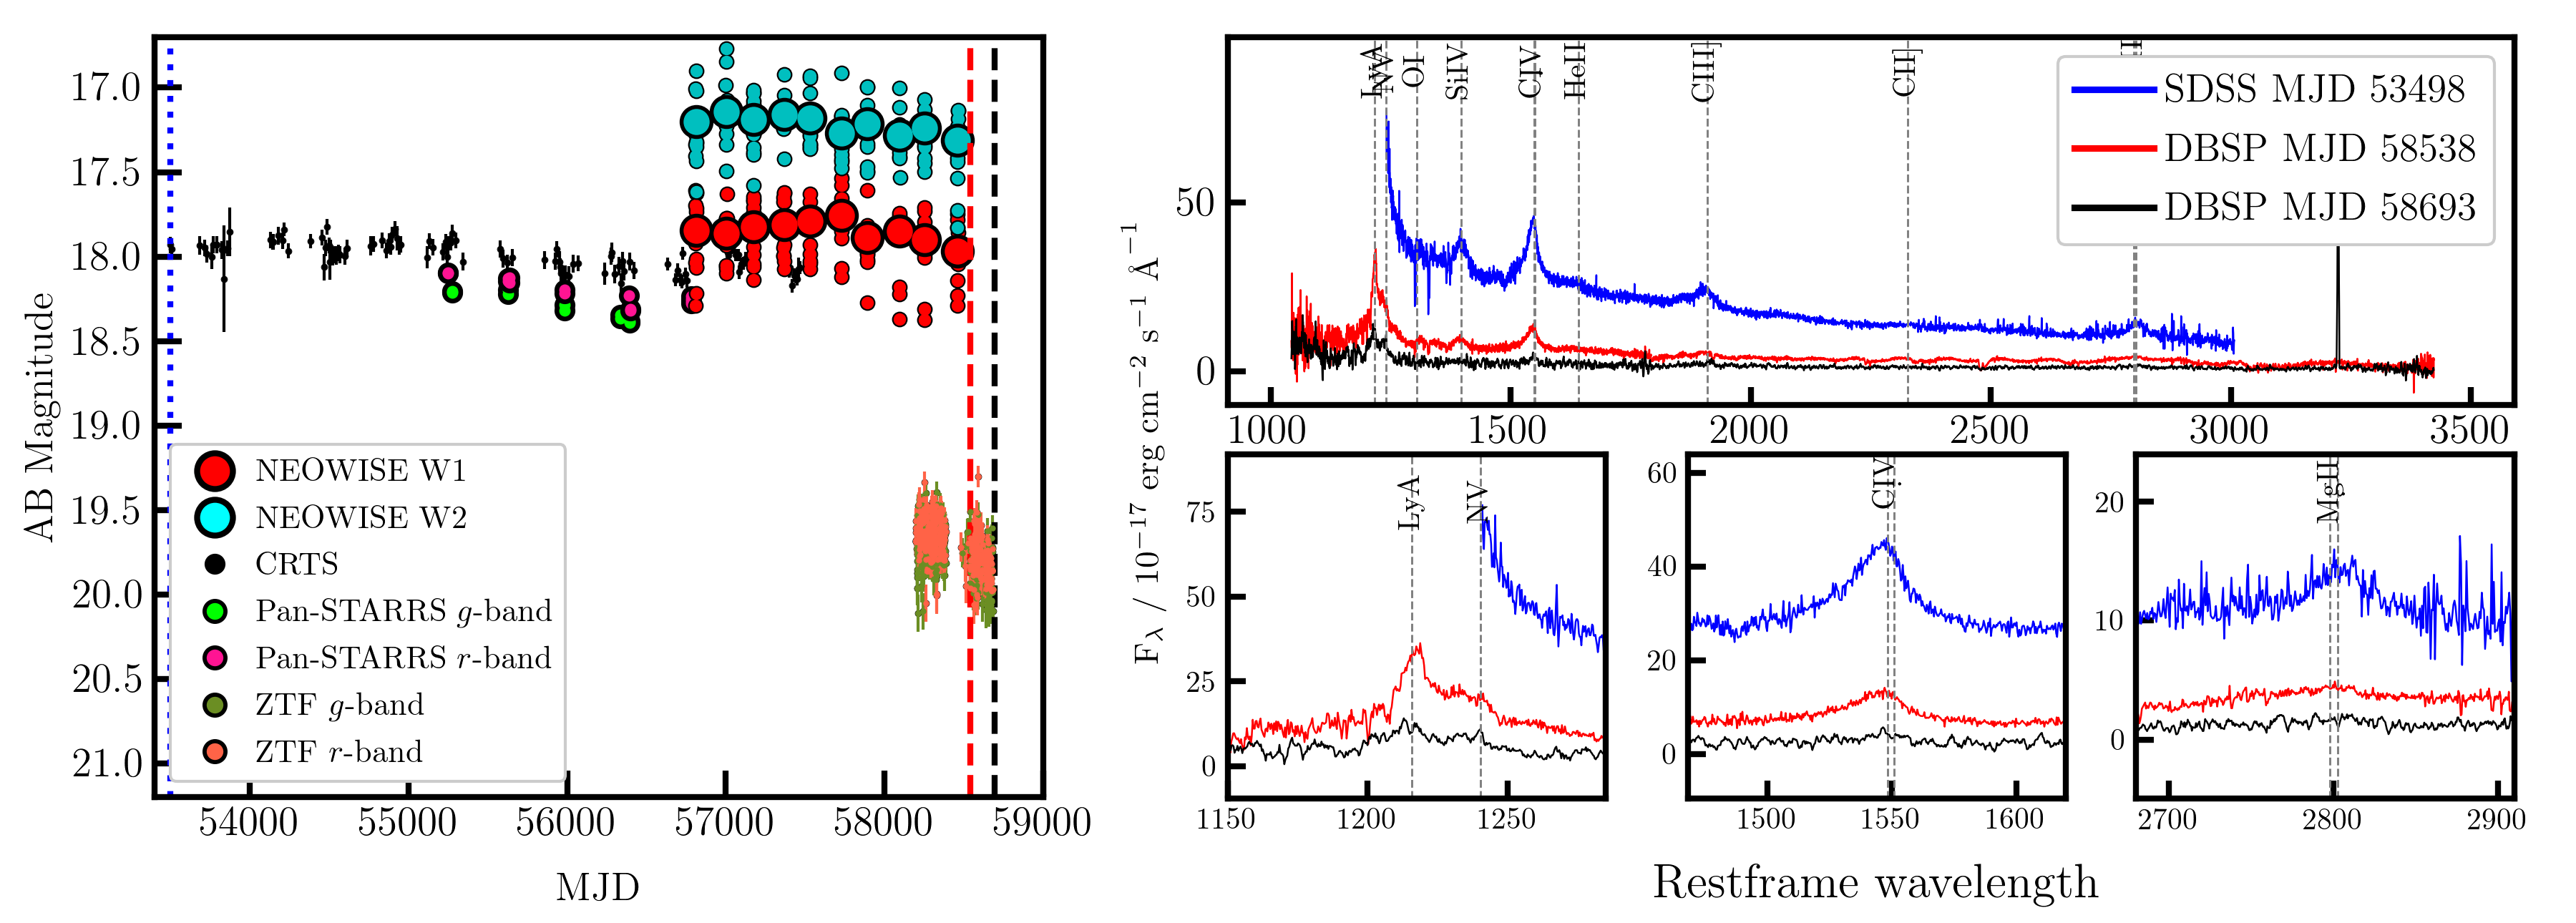
\includegraphics[width=16.7cm, trim=0.3cm 0.05cm 0.45cm 0.1cm, clip]
  {figures/J1205+3422_landscape_20191112.png}
  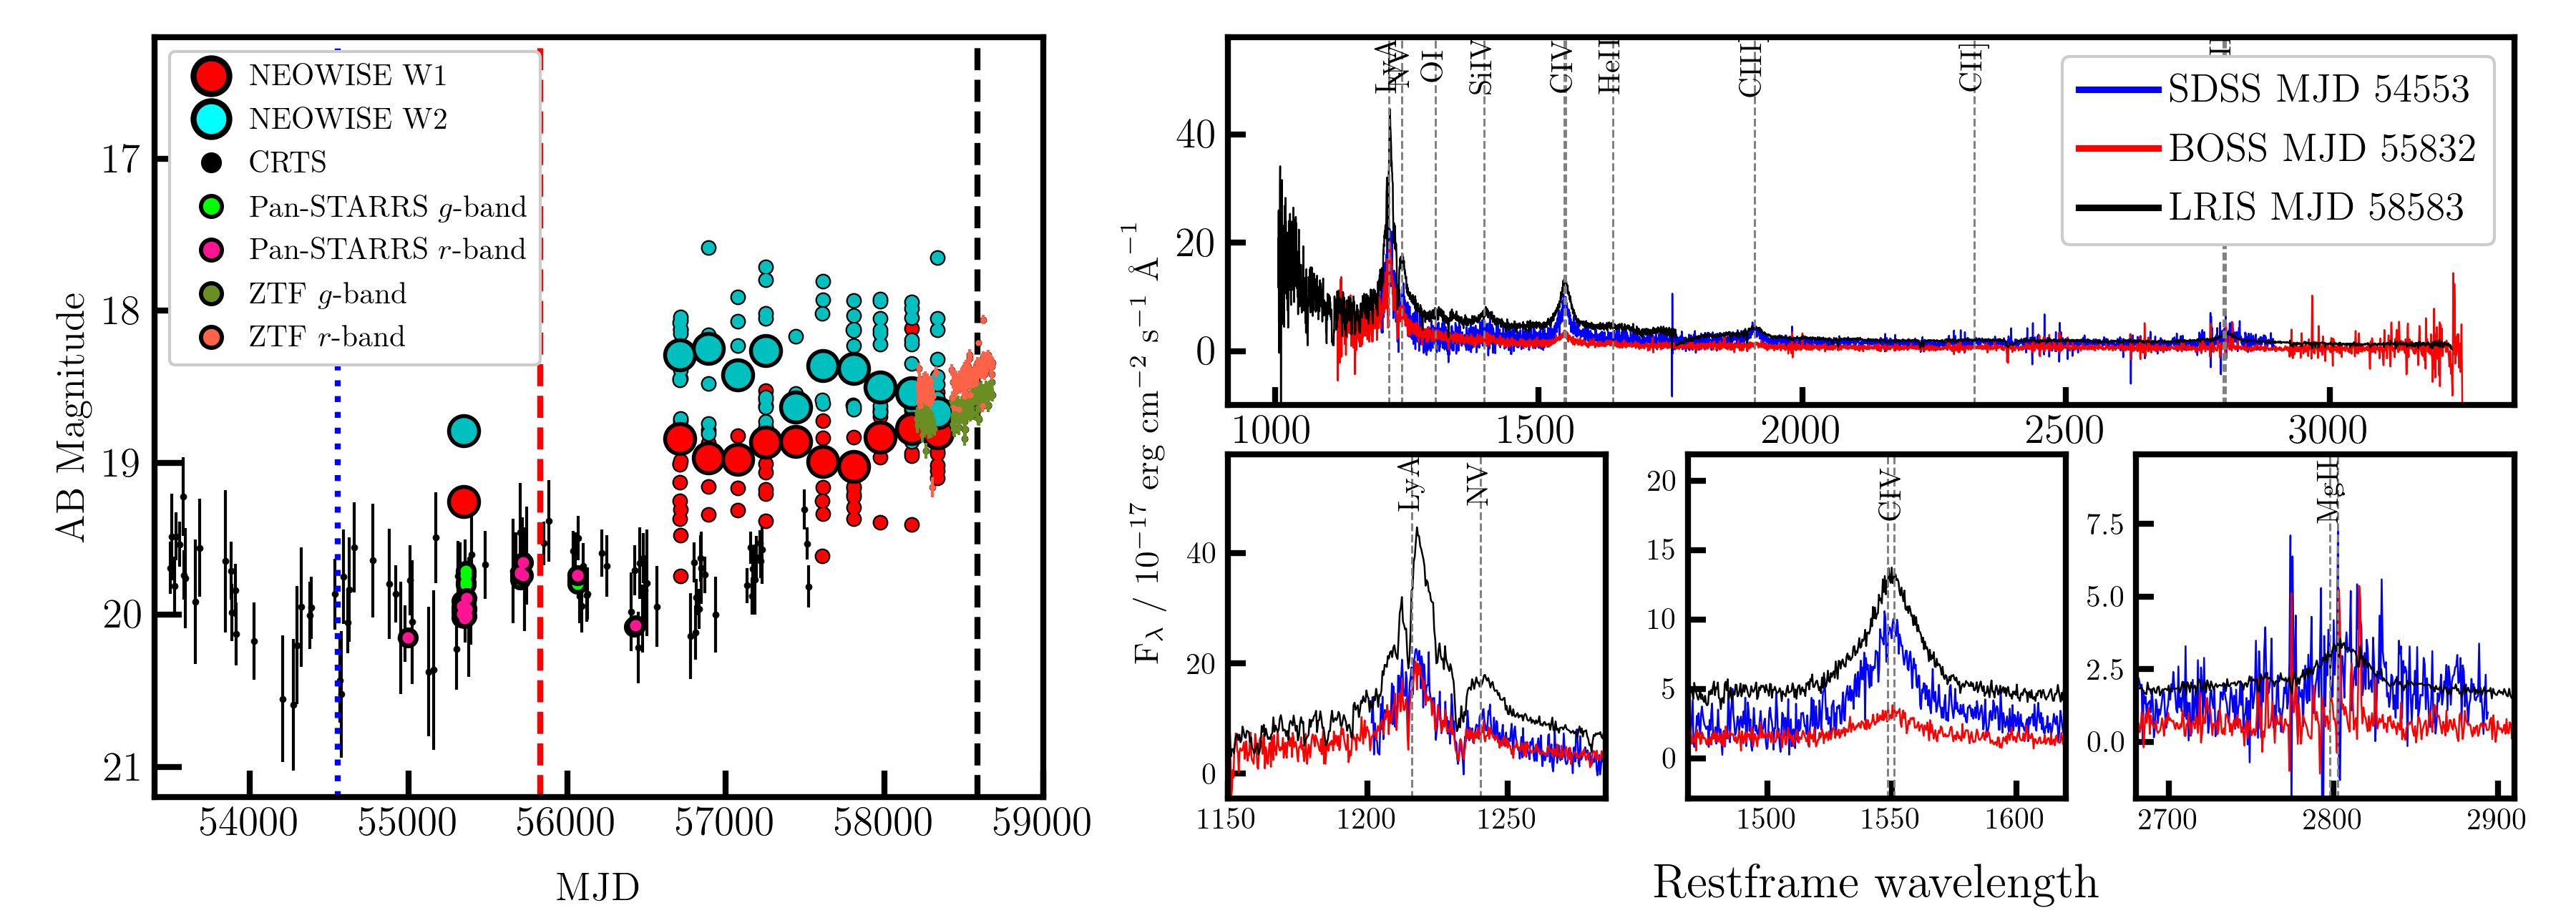
\includegraphics[width=16.7cm, trim=0.3cm 0.05cm 0.40cm 0.1cm, clip]
  {figures/J1638+2827_landscape_20191112.png}
  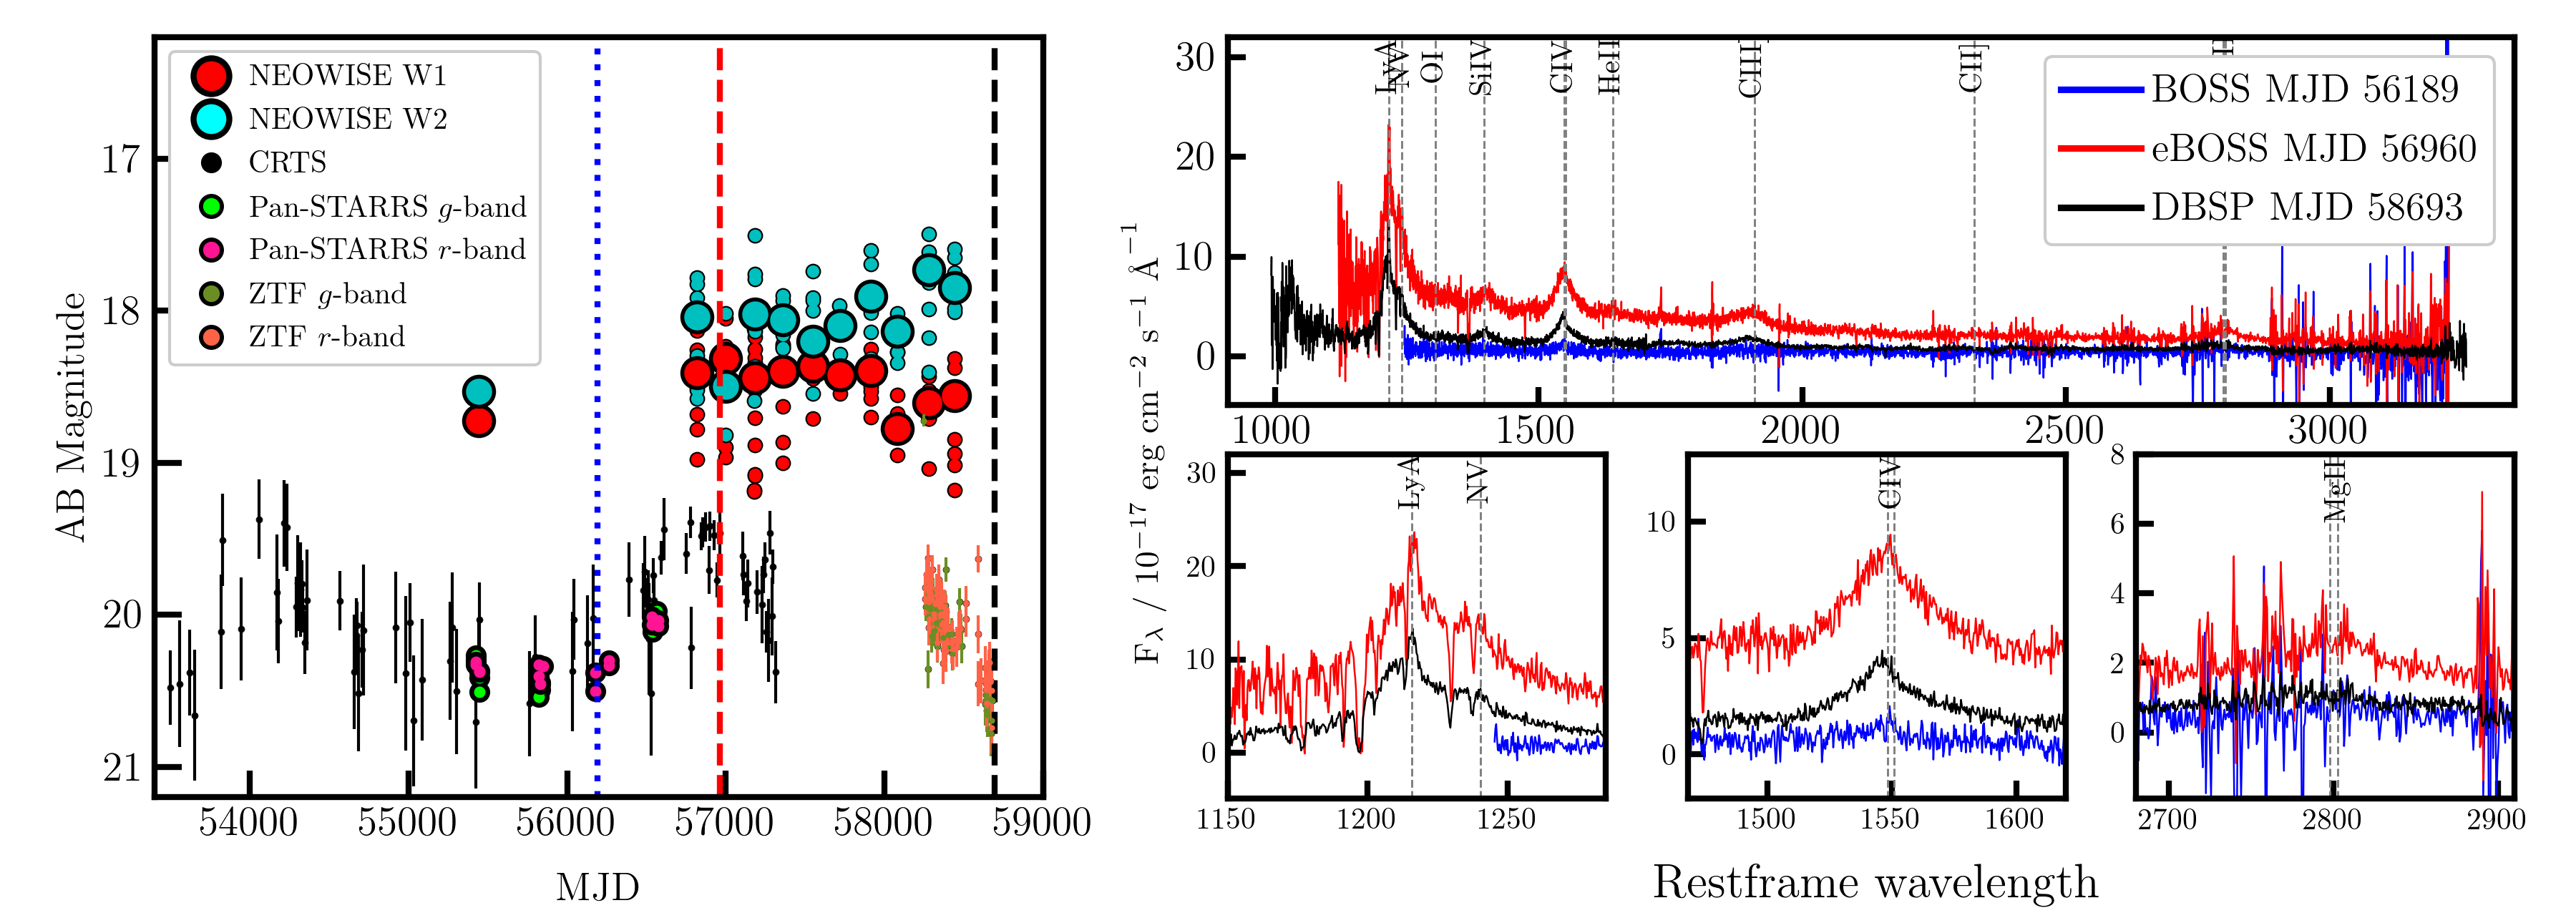
\includegraphics[width=16.7cm, trim=0.3cm 0.0cm  0.35cm 0.1cm, clip]
  {figures/J2228+2201_landscape_20191112.png}
  \vspace{-12pt}
  \caption[]{The three high-$z$ CLQ quasars; 
    J1205+3422 (top), 
    J1638+2827 (middle) and  
    J2228+2201 (bottom). 
The light curve data is present in the panels on the left hand side, with the 
spectral epoch observational timings indicated by vertical lines. 
The spectra are on the right hand side, with zoom-in's on the Ly$\alpha$-\nv 
complex, the \civ\ line, and the \mgii line. 
  }
  \label{fig:civ_clqs}
\end{figure*}
\subsection{Spectroscopy}
An overview of our spectroscopic observations is given in
Table~\ref{tab:obs_notes}.  The spectra are from the SDSS
\citep{Stoughton2002, DR7, Schneider2010}, the SDSS-III Baryon
Oscillation Spectroscopic Survey \citep[BOSS; ][]{Eisenstein2011,
Dawson2013, Smee2013, Alam2015, Paris2017} and the SDSS-IV Extended
Baryon Oscillation Spectroscopic Survey \citep[eBOSS; ][]{Dawson2016,
Abolfathi2018, Paris2018}.  These quasars were targetted via a range
of techniques and algorithms \citep[see ][]{Richards2002, Ross2012,
Myers2015}. The SDSS, BOSS, and eBOSS data are supplemented by
spectra from the Low Resolution Imaging Spectrometer \citep[LRIS; ][]{Oke1995} on the 10m
Keck {\sc I} telescope.  and the Double Spectrograph
(DBSP) instrument on the 200'' Palomar telescope.

\subsubsection{Spectrophotometry}
{\bf MJG to finish this::} \\
We want all our spectra to have reliable flux calibrations.  SDSS
spectra ae spectrophotometrically calibrated.  BOSS and eBOSS spectra
have spectrophotometric corrections applied in the latest data release
\citep{Hutchinson2016, Jensen2016, Margala2016}.  Due to the high-$z$
of our objects, \oiii is not available to us to use as a calibrating
flux line. Instead we use photometric data from the ZTF since all our
non-SDSS/BOSS/eBOSS data are taken after MJD 57500.


\subsection{Emission Line and Power-law Slope Measurements}
We use the measured quasar emission line properties from several catalogues: 
\citet{Shen2011}, \citet{Hamann2017}, \citet{Kozlowski2017}, and
\citet{Calderone2017}.

In particular we use the Quasar Spectral Fitting (QSFit) software
package presented in \citet{Calderone2017}. This provides luminosity
estimates as well as width, velocity offset and equivalent width of 20
emission lines, including \civ, \ciii and \mgii.  We process and fit
all nine spectra using the lastest version (v1.3.0) of the QSFit 
\href{https://qsfit.inaf.it/cat_1.30/onlinefit.php}{online
calculator}.
% and setting $E(B-V)=0.00$.
%%
The host galaxy and blended iron emission at rest-frame optical
wavelengths components are automatically disabled when they can not be
constrained by the available data, such as the case for all our
objects (we do not have infrared spectral data).
%%
Power-law continuum slopes, $\alpha$, where $f_{\lambda} \propto
\lambda^{\alpha}$, are also reported in these catalogues and from
QSFit.  We quote the most appropriate value given the emission line
wavelength.




%%%%%%%%%%%%%%%%%%%%%%%%%%%%%%%%%%%%%%%%%%%%%%%%%%%%%%%%%%%%%%%%%%%%%%%%%%%%%
%%%%%%%%%%%%%%%%%%%%%%%%%%%%%%%%%%%%%%%%%%%%%%%%%%%%%%%%%%%%%%%%%%%%%%%%%%%%%
%%
%%   SECTION 3   SECTION 3   SECTION 3   SECTION 3   SECTION 3   SECTION 3  
%%   SECTION 3   SECTION 3   SECTION 3   SECTION 3   SECTION 3   SECTION 3  
%%   SECTION 3   SECTION 3   SECTION 3   SECTION 3   SECTION 3   SECTION 3  
%%
%%%%%%%%%%%%%%%%%%%%%%%%%%%%%%%%%%%%%%%%%%%%%%%%%%%%%%%%%%%%%%%%%%%%%%%%%%%%%
%%%%%%%%%%%%%%%%%%%%%%%%%%%%%%%%%%%%%%%%%%%%%%%%%%%%%%%%%%%%%%%%%%%%%%%%%%%%%
\section{Results}
\subsection{Photometric and Spectral Evolution}
Figure~\ref{fig:civ_clqs} presents the optical and mid-IR light
curves for three high-$z$ CLQ quasars.  Figure~\ref{fig:civ_clqs} also
shows the spectra for each epoch, with the MJD of observation given by
the dashed vertical lines in the light curves.

For J1205+3422, our spectral observations cover 5195 days observed,
1691 days in the rest-frame. This quasar was initially identified in
SDSS in 2005 May, as a bright, $g\approx18.0$, blue-sloped quasar with
broad \siiv, \civ, \ciii and \mgii. \ciii and \civ\ have large
blueshifts of $\approx$2600$\pm$150 and $\approx$1150$\pm$100 km
s$^{-1}$, respectively.  By 2019, however, the opitical brightness
dropped by $\sim$1.5 magnitudes and the spectra are significantly less
blue.  While \lya and \nv are detectable in both 2019 spectra, \civ\
has all but disappeared in the 2019 June spectrum.  The broad \ciii
emission has disappeared between the 2005 and 2019 spectra. The
changes in \civ\ and \ciii going from broad emission to barely
detectable have on the timescales of $\approx$50 days in the
rest-frame.

For J1638+2827, our spectral observations cover 4030 days observed,
1265 days in the rest-frame. Here, in the initial epoch spectrum,
\civ\ is broad and bright, as is C\,{\sc iii}. However, $\approx$400
rest-frame days later, the broad \civ\ and \ciii BEL have faded, the
continuum slope around 1400\AA\ has changed from $\approx-1.48$ to
$\approx-2.25$, but the \lya/\nv emission complex is very similar in
shape and line flux intensity. Around 870 days in the rest-frame after
the second spectral epoch, \lya, \nv, \civ, \ciii and \mgii are all
apparent and broad, with \mgii being seen for the first time at high
signal-to-noise. The light curve is consistent with this spectral
brightening, increasing from $\sim$20th magnitude to $\sim$18.5
magnitude at optical wavelengths. An absorption feature between \lya
and \nv is seen in all three spectral epochs.

For J2228+2201, our spectral observations cover 2504 days observed,
778 days in the rest-frame. Over the course of 240 rest-frame days,
\civ\ and \ciii both {\it emerge} as BELs and the standard UV/blue
continuum slope increases in flux.  Then, over the course of 538 days
in the rest-frame, the broadline emission, while still very present,
reduces in line flux the UV/blue continuum diminishes, though is still
more luminous than the initial BOSS spectrum.

\begin{figure}
  \centering
  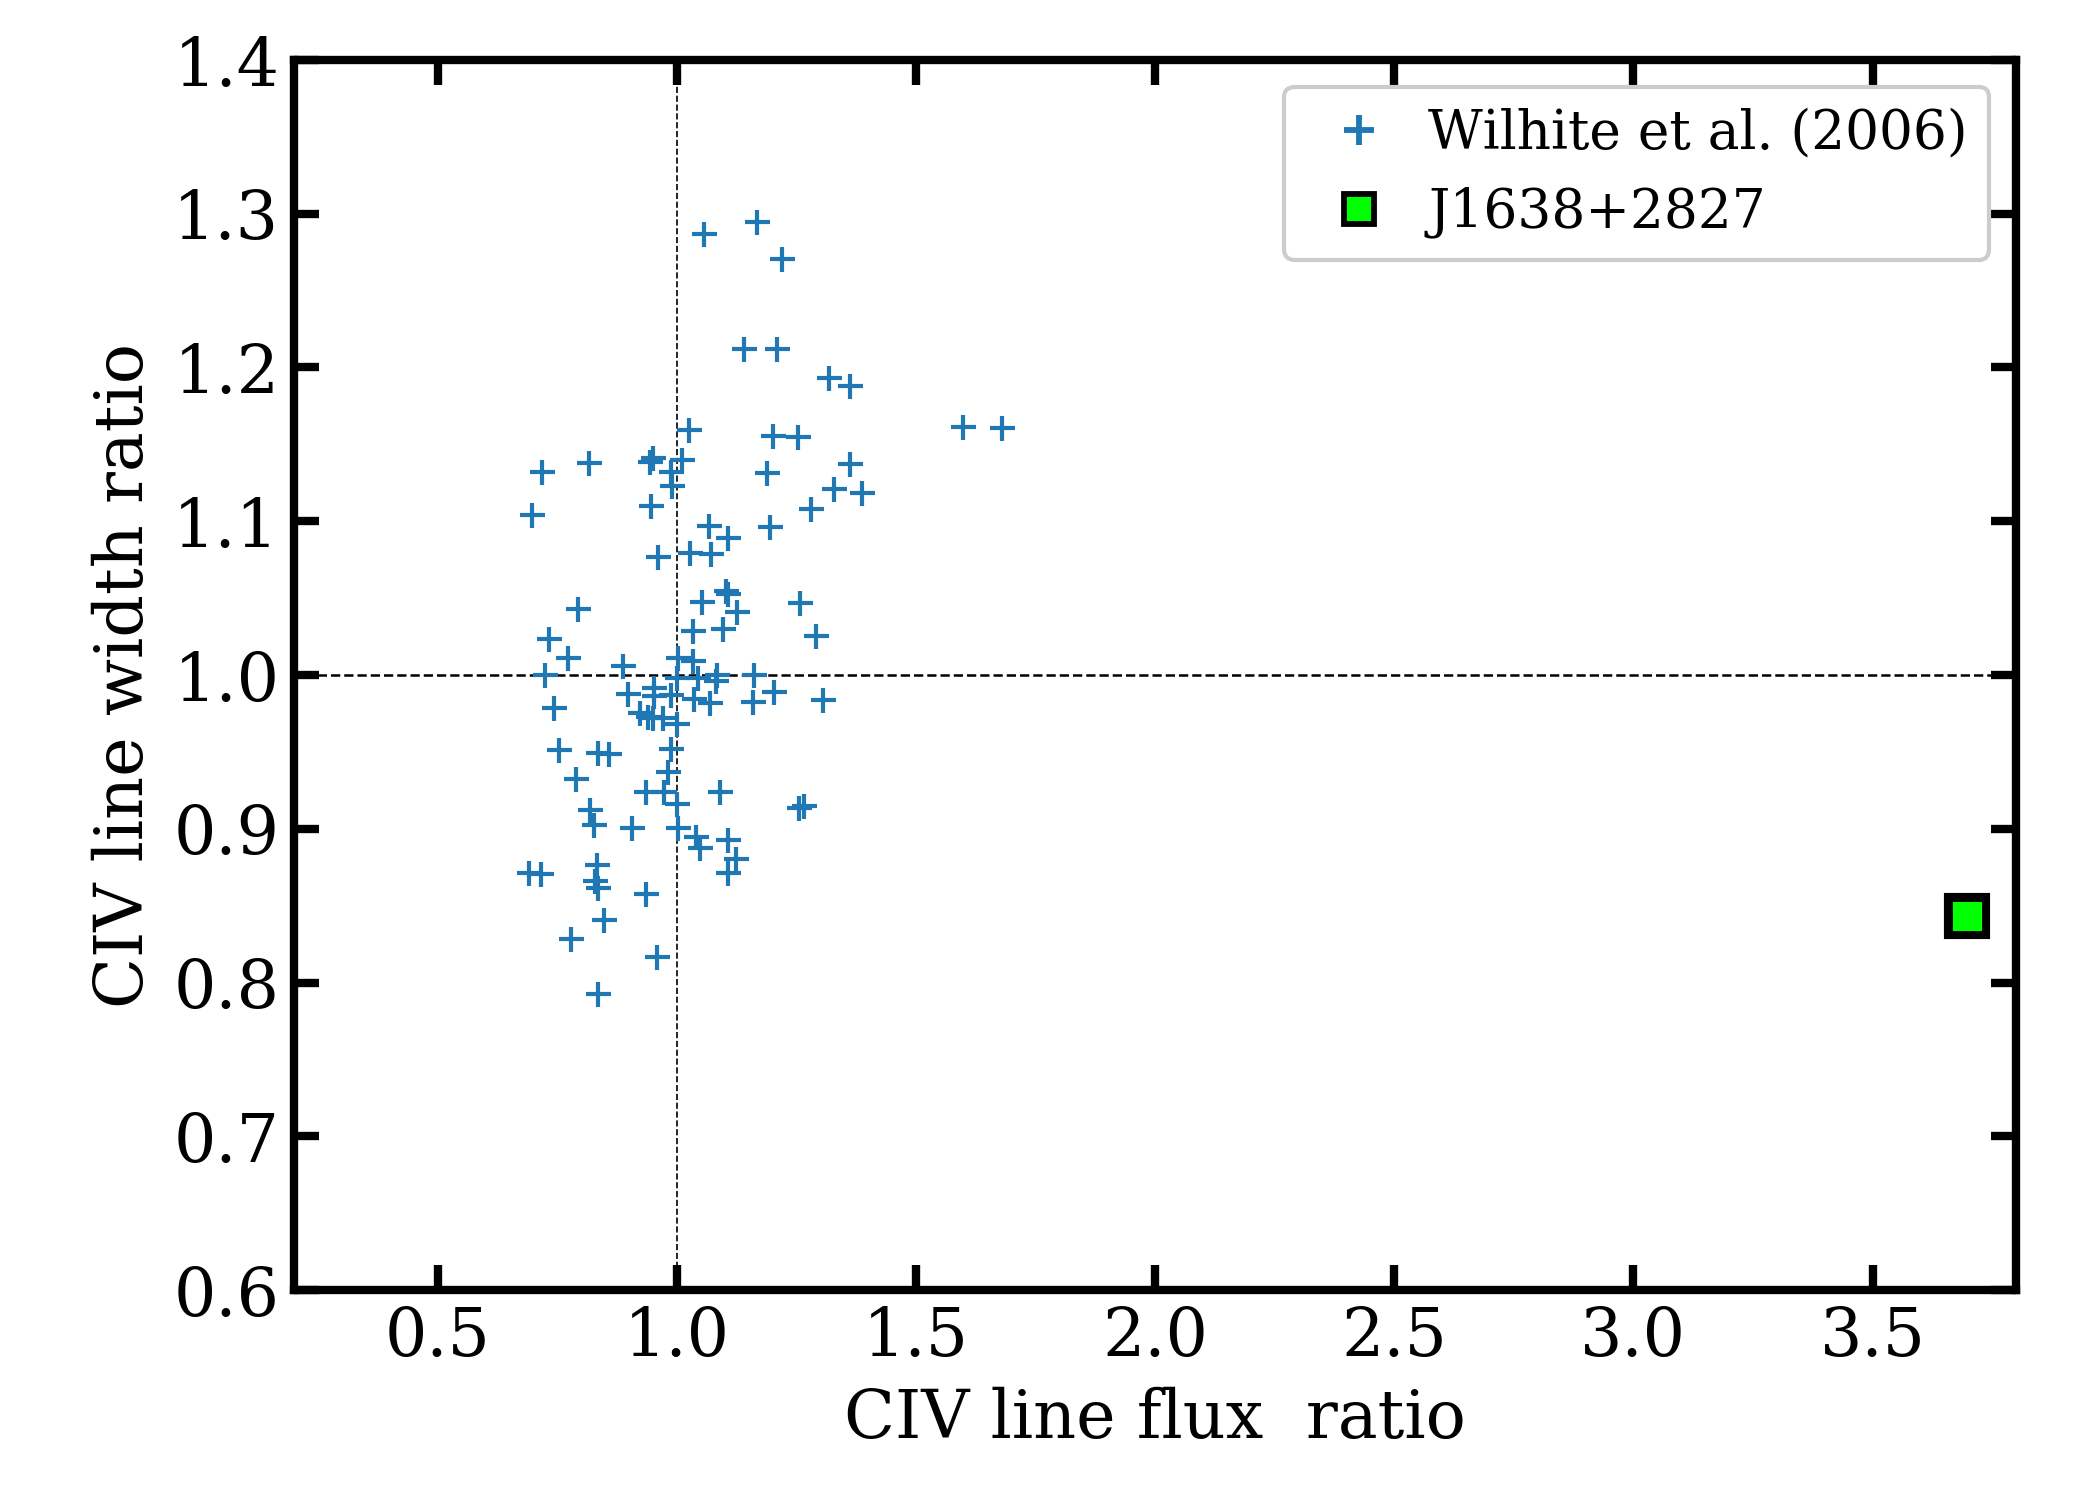
\includegraphics[width=8.7cm, trim=0.2cm 0.2cm 0.2cm 0.2cm, clip]
  {figures/Wilhite_2006_Fig2_redux_20190926.png}
   \vspace{-12pt}
  \caption[]{The Change in \civ\ line width vs. line flux change. 
We compare our object J1638+2827 with the sample 
from \citet{Wilhite2006} with a sample of 105 quasars observed at
multiple epochs by the SDSS. J1638+2827 is a substantial outlier 
in this parameter space.}
  \label{fig:Wilhite2006_comparison}
\end{figure}
\subsection{Emission Line Evolution}
Emission line measurements from the catalogues of \citet{Shen2011}.
\citet{Hamann2017}, \citet{Kozlowski2017} or the QSFit routine of
\citet{Calderone2017} are presented in Table~\ref{tab:LineMeasurements}.

From Figure~\ref{fig:Wilhite2006_comparison} there appears to be a
strong correlation between the change in the line flux and the change
in the line width.  Figure~\ref{fig:Wilhite2006_comparison} shows the
epoch-to-epoch flux ratio versus the ratio of line widths.

For the BOSS spectrum of J2228+2201 on MJD 56189, some of the data are
``masked'' (i.e. they have {\tt and\_mask} != 0) in the FITS file at
wavelengths $\lesssim$1600\AA\ (rest-frame).  This typically means
there is some potential problem in using those data. However, visual
inspection shows strong broad \civ\ emission, so we disable the check on the mask,
and report the line fits in Table~\ref{tab:LineMeasurements} and show the \civ\ line 
fits in~\ref{fig:CIV_LineFits}.

\begin{figure}
  \centering
  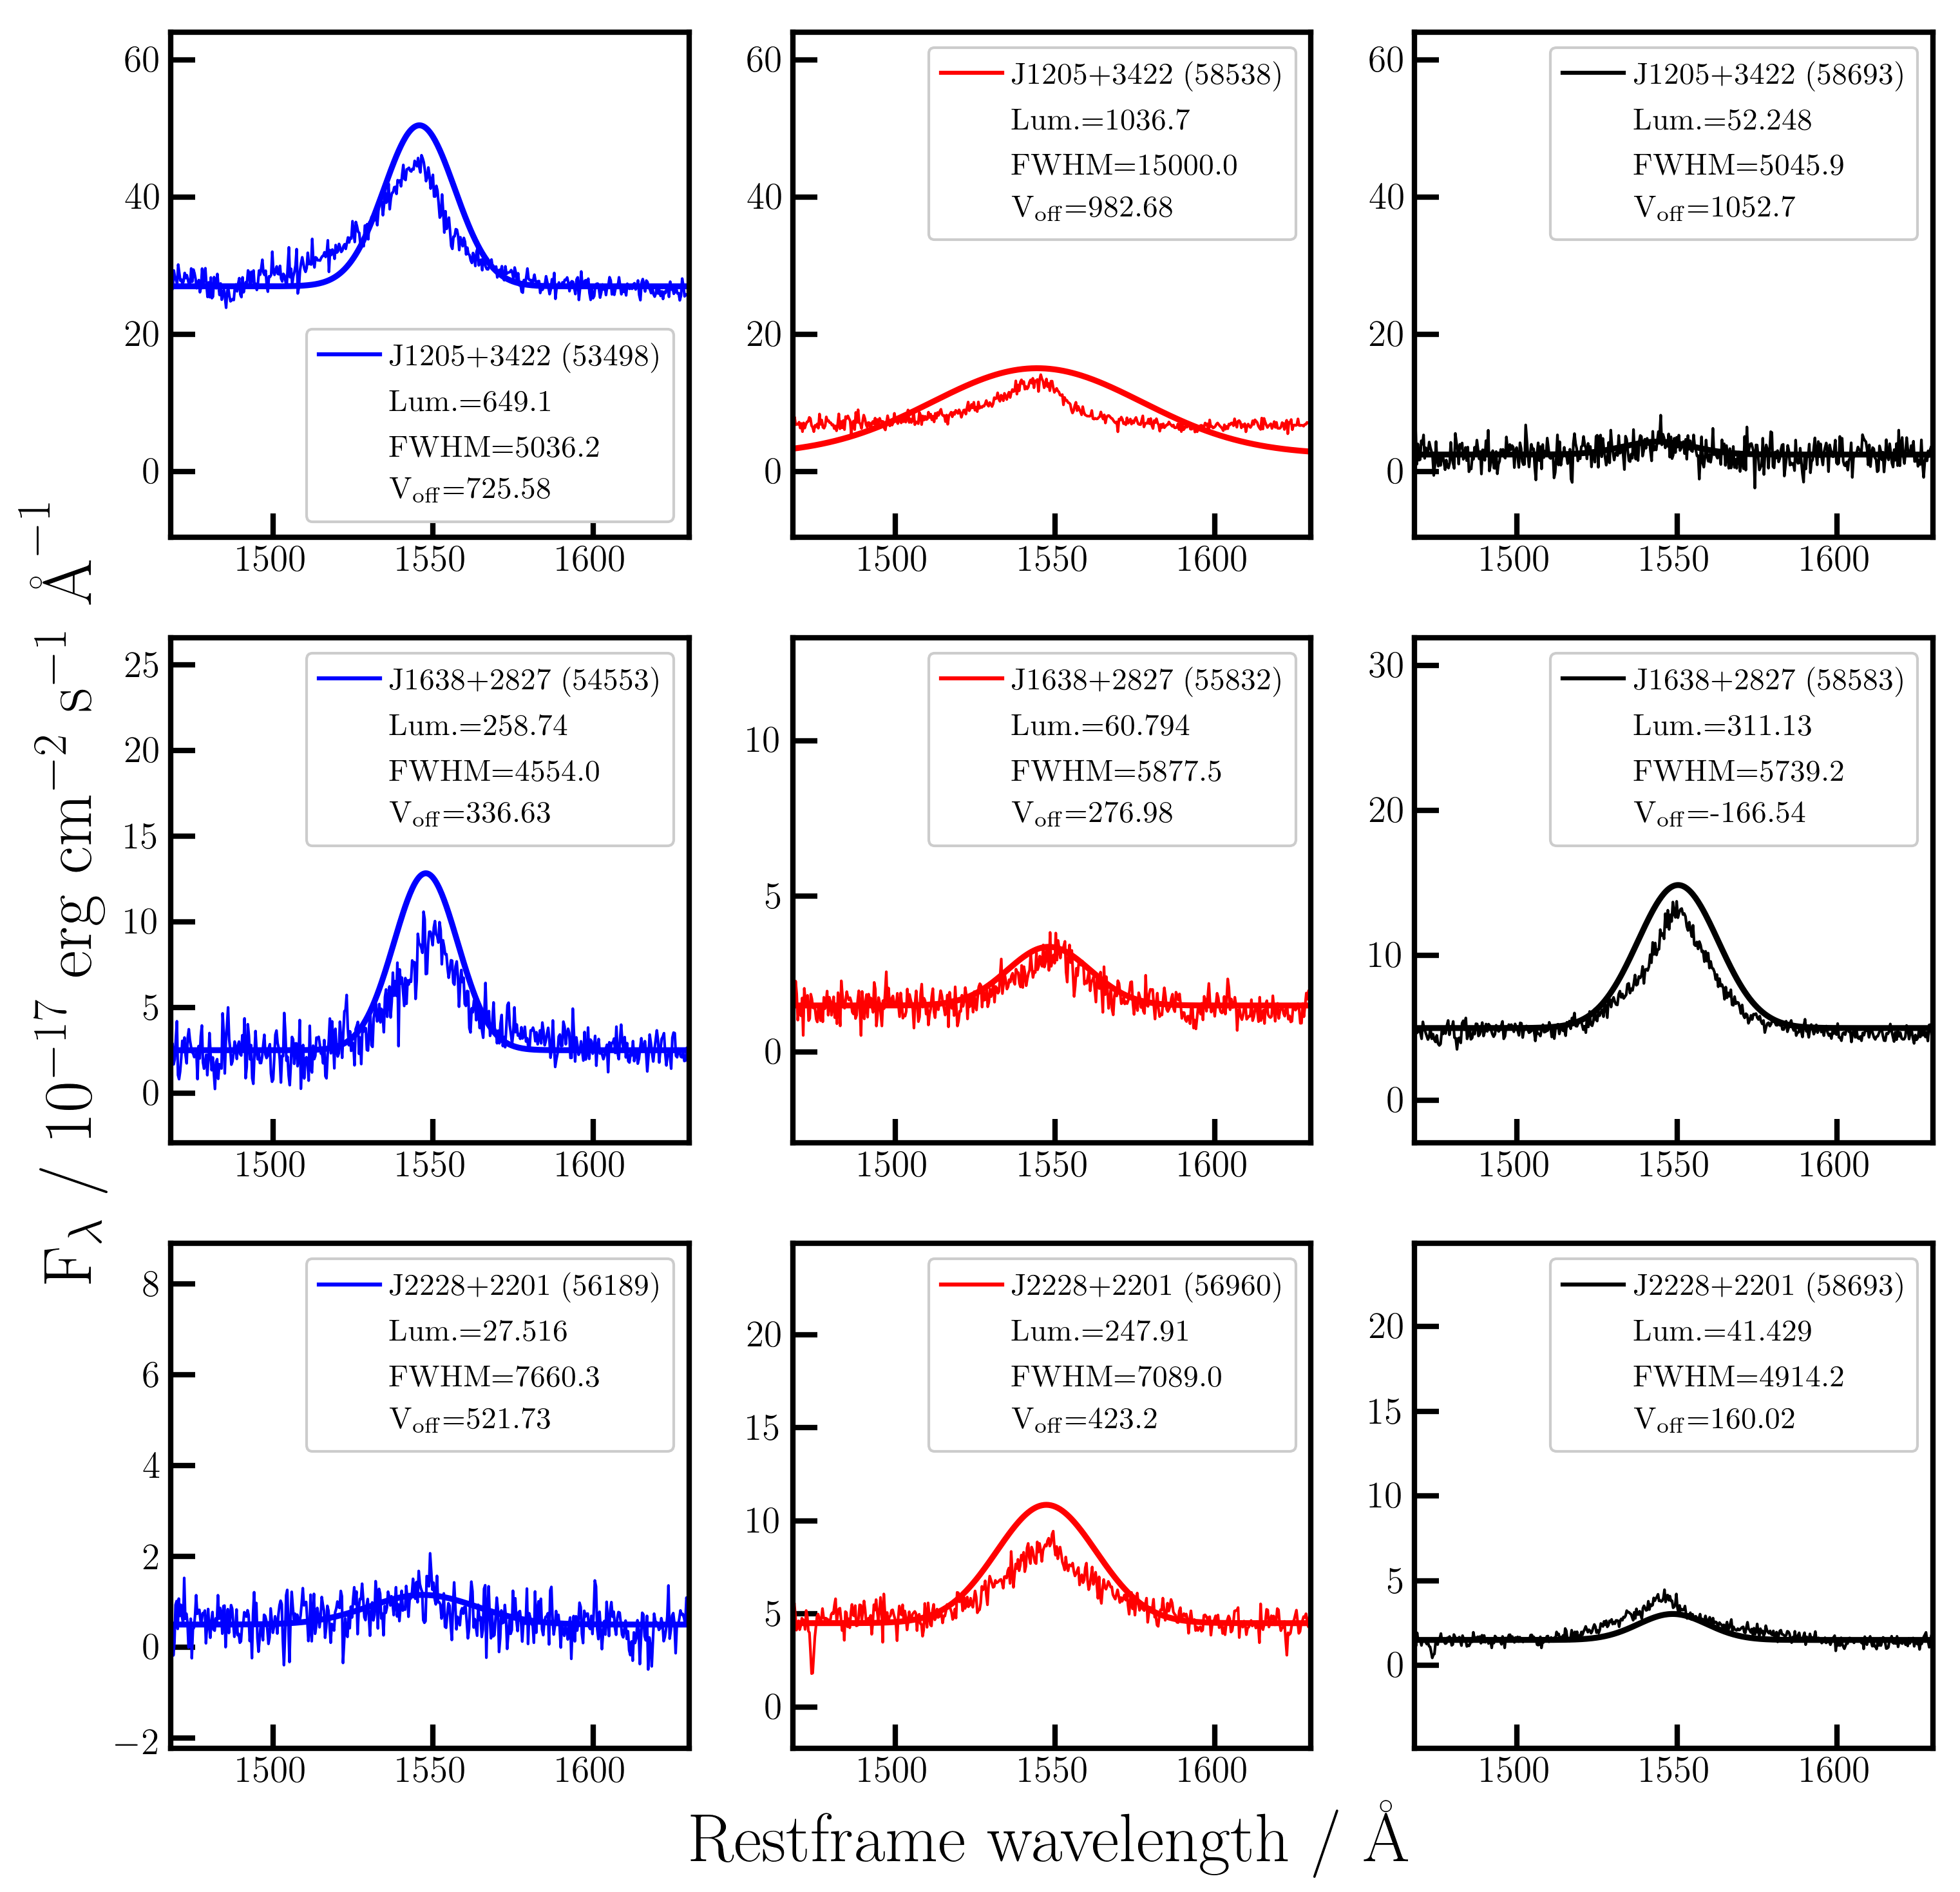
\includegraphics[width=8.5cm, trim=0.4cm 0.4cm 0.2cm 0.4cm, clip]
  {figures/CIV_fits_20191108.png}
   \vspace{-12pt}
   \caption[]{The \civ\ emission line and the subsequent QSFit model and
     parameters.}
   \label{fig:CIV_LineFits}
\end{figure}

\begin{table*}
  \centering
  %   \begin{tabu}{l ll  ll cc c r }
    \hline 
    \hline 
    Object                               &   MJD      & line      & Line  Lumin.     &   FWHM                       &  $V_{\rm off}$         & E.W.                          & $\alpha_{\lambda}$  &   Catalogue \\                                   
    \hline                                     
    \rowfont{\color{blue}}       & 53498    & \civ      &  511$\pm$13    &   9593$\pm$287        &  1172$\pm$74      & 15.9$\pm$0.4      & $-1.64\pm0.01$       &  QSFit         \\    %% (NPR) 
    \rowfont{\color{blue}}       & 53498    & \civ      &  787                   &   5230$\pm$219        &  1118$\pm$133    & 30.1$\pm$1.21    & $-1.47\pm0.08$       &  Shen2011 \\
    \rowfont{\color{blue}}       & 53498    & \civ      &   403                  &   5119$^{(a)}$             &    ---                     &  ---                        &  ---                         &  DR12 SAS   \\
                                             & 53498     & \ciii      &  441$\pm$10   & 14959$\pm352^{(b)}$ &  2616$\pm$147    & 25.10$\pm$0.59    & $-1.65\pm0.01$      &  QSFit          \\  %% (NPR) 
                                             & 53498    & \ciii       &   144                 &   5119$^{(a)}$             &  ---                       &   ---                       &  ---                          &  DR12 SAS  \\
  \rowfont{\color{teal}}         & 53498     & \mgii     &  327$\pm$20   &   4907$\pm$387       &  $-274\pm419$     & 26.66$\pm$1.65    &   $-1.65\pm0.01$    &  $^{(d)}$QSFit  \\  %% (NPR) 
  \rowfont{\color{teal}}         & 53498     & \mgii     &  284                  &   4730$\pm$314       &  $-179\pm188$     & 32$\pm$3.88         &  $-1.87\pm0.06$     &  Shen2011 \\
 \multirow{2}{*}{{\bf J1205+3422}}  
                &     \textcolor{teal}{53948}     & \textcolor{teal}{\mgii}   & \textcolor{teal}{130} & \textcolor{teal}{5119$^{(a)}$}   &  \textcolor{teal}{---}   & \textcolor{teal}{---}        & \textcolor{teal}{---}    & \textcolor{teal}{DR12 SAS}    \\
                                 \cdashline{2-9}
                                            & 58538     & \lya      & 952$\pm$1.1    & 12242$\pm$15    &  $-1679\pm6$          &  165$\pm$0.2        &  ---                       &   QSFit  \\    %% (MJG)
   \rowfont{\color{blue}}       & 58538     & \civ      & 1037$\pm$5    & $>$15000             &  983$\pm$40            &  ---                        &  ---                       &   QSFit  \\   %% (NPR) 
                                            & 58538      & \ciii     &  167$\pm$0.9  & $>$15000            &  2734$\pm$46            &     45$\pm$0.2       &  ---                       &  QSFit  \\    %% (MJG)
    \rowfont{\color{teal}}      & 58538     & \mgii    &  216$\pm$1.4  & 13940$\pm$94    & $-465.2\pm38$         &  88$\pm$0.6	    &  ---                       &   QSFit  \\    %% (MJG)
                                          \cdashline{2-9}
                                           & 58693     & \lya     &  271$\pm$0.9    & 9637$\pm$52     &  $-447\pm13$          &  85.1$\pm$0.3          & ---                        &   QSFit  \\    %% (MJG)
    \rowfont{\color{blue}}    & 58693     & \civ      &   52$\pm$0.9    & 5046$\pm$26     &   1053$\pm$17         &   24.0$\pm$0.2          & ---                        &  QSFit \\     %% (MJG)
                                           & 58693     & \ciii     &   59$\pm$0.9    & 10751$\pm$        &  1097$\pm$77         &   36$\pm$0.6             & ---                        &  QSFit   \\    %% (MJG)
   \rowfont{\color{teal}}      & 58693     & \mgii    &  69$\pm$1.5    & 14983$\pm$346   &  $-190\pm134$       &    72$\pm$1.6           & ---                        &  QSFit   \\    %% (MJG)
\hline
                                                & 54553     & \lya      & 188                 &  3207                     &    ---                        &   ---                         & ---                    &   DR12 SAS  \\
   \rowfont{\color{blue}}          & 54553     & \civ      & 257$\pm$13   &  4550$\pm$371     &   55$\pm$450         &   31.8$\pm$1.5     &                                &  $^{(d)}$QSFit  \\   %% (NPR) 
   \rowfont{\color{blue}}          & 54553     & \civ      & 281                  &    4181$\pm$736   &    680$\pm$133       & 100.5$\pm$12  & $-0.14\pm0.68$        &  Shen2011   \\
   \rowfont{\color{blue}}          & 54553     & \civ      & 170                  &   4537$^{(a)}$        &    ---                       &   ---                         & ---                         &  DR12 SAS  \\    %% (NPR) 
                                                & 54553     & \ciii     &  130$\pm$10   &  3852$\pm$402    &  $-236\pm565$       &  36.7$\pm$2.8          &  $-1.47\pm0.20$    &  $^{(d)}$QSFit  \\
                                                & 54553     & \ciii     &  61                    &  4537$^{(a)}$          &  ---                         &  ---                           & ---                         &  DR12 SAS \\    %% (NPR) 
    \rowfont{\color{teal}}          & 54553      & \mgii  &  139                  &  4757$\pm$2224   &  $-944\pm568$        &   119$\pm$40          &  $-1.49\pm0.54$    &  Shen2011   \\
    \rowfont{\color{teal}}          & 54553      & \mgii  &  69                    &  4537$^{(a)}$           &    ---                        &  ---                          & ---                          &  DR12 SAS  \\   %% (NPR) 
                                                \cdashline{2-9}
                                                & 55832     & \lya     & 288$\pm$11    &  4444$\pm$243       &  -463$\pm$68         &  103.69$\pm$3.99   &                               &   QSFit  \\
                                                & 55832     & \lya     & 234                  &  4165.6$^{(a)}$         &    ---                       &   ---                         & ---                         &   DR12 SAS  \\    %% (NPR) 
\multirow{2}{*}{\bf {J1638+2827}}
 & \textcolor{blue}{55832} & \textcolor{blue}{\civ}    & \textcolor{blue}{63$\pm$3}  &   \textcolor{blue}{6052$\pm$250}  &  \textcolor{blue}{-117$\pm$103}  &  \textcolor{blue}{43.2$\pm$1.7}  &  \textcolor{blue}{-2.25$\pm$0.05} & QSFit    \\
    \rowfont{\color{blue}}           &  55832   &  \civ     &  ---               &    5210$\pm$226     &    ---                       &   42.8$\pm$2.0         & $-3.35$                 &     Ham17  \\
    \rowfont{\color{blue}}           &  55832   &  \civ     &  46                 &    5385$^{(a)}$           &    ---                       &   ---                         & ---                         & DR12 SAS \\
                                                 & 55832     & \ciii     & 15$\pm$5     &  11421$\pm$3654   &   $>$3000                &   14.8$\pm$4.5         &  $-2.25\pm0.05$   &        QSFit \\
                                                 &  55832    &  \ciii    &  11                 &     5385$^{(a)}$         &  ---                          &    ---                         &  ---                       &   DR12 SAS \\  
    \rowfont{\color{teal}}           &  55832     & \mgii   &  13                &     5385$^{(a)}$         &  ---                           &   ---                          &  ---                       &   DR12 SAS\\  
                                               \cdashline{2-9}
                                               & 58583       & \lya    &  785$\pm$1      & 4956$\pm$4    	&   $-641\pm2$            &   90$\pm$0.1   	  &  ---                          &  QSFit  \\ %% (MJG)
   \rowfont{\color{blue}}         & 58583      & \civ      &  311$\pm$1     & 5739$\pm$14	 &  $-167\pm6$             &   58$\pm$0.1          & ---                          &   QSFit  \\  %% (MJG)
                                               & 58583      & \ciii      &  52$\pm$0.8   &  3917.4	68.837      &  1514$\pm$127        &  124$\pm$2             & ---                          &   QSFit \\   %% (MJG)
   \rowfont{\color{teal}}           & 58583      & \mgii   &  157$\pm$2    &  10565$\pm$129    &  $-450\pm52$          &   92$\pm$1              & ---                          &   QSFit  \\  %% (MJG)
\hline
    \rowfont{\color{blue}}         &  56189     & \civ    &   32$\pm$3.5   &   7663$\pm$881       &    538$\pm$352       &   50.2$\pm$5.6      & ---                        &    QSFit  \\
    \rowfont{\color{blue}}         &  56189     & \civ    &   ---                 &   2994$\pm$620       &     ---                       &   42.2$\pm$5.6      & -1.59                      &    Ham17  \\
    \rowfont{\color{blue}}         &  56189     & \civ    &   19                  &    5218$^{(a)}$            &    ---                       &   ---                       &  ---                        &   DR12 SAS  \\
                                               &  56189      &  \ciii   &  34$\pm$6       &  13748$\pm$2869    &   1851$\pm$1140    &  63$\pm$12          &  $-0.46\pm0.21$    &   QSFit  \\
                                               &  56189      & \ciii    &  7                     &     5218$^{(a)}$          &  ---                         &     ---                     & ---                         &   DR12 SAS \\  
    \rowfont{\color{teal}}          & 56189      & \mgii  &  25$\pm$6       &   7253$\pm$1712     &   $-931\pm708$      &  51$\pm$10.95      &  $-0.46\pm0.21$   &   QSFit   \\
    \rowfont{\color{teal}}         &  56189      &  \mgii &  13                   &     5218$^{(a)}$          &  ---                         &   ---                        &  ---                       &   DR12 SAS \\  
                                                  \cdashline{2-9}
                                              & 56960         & \lya    & 121$\pm$38     & 3580$\pm$673       &     -16$\pm$171     &  13.52 $\pm$4.21    & ---                        &   QSFit   \\  
\multirow{2}{*}{{\bf J2228+2201}}
           & \textcolor{blue}{56960} & \textcolor{blue}{\civ}  & \textcolor{blue}{229$\pm$4}      &  \textcolor{blue}{8911$\pm$169}   &   \textcolor{blue}{92$\pm$68}  &   \textcolor{blue}{46.8$\pm$0.9}    & ---    & \textcolor{blue}{QSFit}     \\   
                                               & 56960    & \ciii      & 185$\pm$5        &        -                      &  2701$\pm$225      &   47.75$\pm$1.29     & ---                      &   QSFit    \\  
   \rowfont{\color{teal}}           & 56960    & \mgii   &   99$\pm$4        &  7312.6$\pm$340   &   188$\pm$137      &   50.75$\pm$2.21     & ---                      &   QSFit   \\
                                               \cdashline{2-9}
                                               & 58693     & \lya      &  447$\pm$5       & 8133$\pm$93       &   613$\pm$130       &        56$\pm$0.6     &  ---                    	 &   QSFit  \\%% (MJG)
     \rowfont{\color{blue}}        & 58693     & \civ      &  41$\pm$1        &  4914$\pm>$65    &   160$\pm$27         &   25$\pm$0.3          & ---                         & QSFit   \\  %% (MJG)
                                               & 58693     & \ciii      & 107$\pm$1.2    &  $>$15000             &  2422$\pm$67        &   ---                       & ---                          &  QSFit    \\  %% (MJG)
     \rowfont{\color{teal}}        & 58693     & \mgii    & 177$\pm$1.1    &  $>$15000             &  1000$\pm$2617    &   16$\pm$36         & ---                           &   QSFit  \\  %% (NPR) 
\hline
\hline
    \end{tabu}
  \begin{tabu}{l ll  ll cc c r }
  \hline 
  \hline 
  Object                               &   MJD      & line      & Line  Lumin.     &   FWHM                       &  $V_{\rm off}$         & E.W.                          & $\alpha_{\lambda}$  \\                          
  \hline                                     
  & 53498    & \civ      &  511$\pm$13    &   9593$\pm$287        &  1172$\pm$74      & 15.9$\pm$0.4      & $-1.64\pm0.01$             \\    %% (NPR) 
  & 53498     & \ciii      &  441$\pm$10   & 14959$\pm352^{(b)}$ &  2616$\pm$147    & 25.10$\pm$0.59    & $-1.65\pm0.01$              \\  %% (NPR) 
  & 53498     & \mgii     &  327$\pm$20   &   4907$\pm$387       &  $-274\pm419$     & 26.66$\pm$1.65    &   $-1.65\pm0.01$     \\  %% (NPR) 
  \cdashline{2-9}
  {\bf J1205+3422}
  & 58538     & \lya      & 952$\pm$1.1    & 12242$\pm$15    &  $-1679\pm6$          &  165$\pm$0.2        &  ---                       \\    %% (MJG)
  & 58538     & \civ      & 1037$\pm$5    & $>$15000             &  983$\pm$40            &  ---                        &  ---                        \\   %% (NPR) 
  & 58538      & \ciii     &  167$\pm$0.9  & $>$15000            &  2734$\pm$46            &     45$\pm$0.2       &  ---                        \\    %% (MJG)
  & 58538     & \mgii    &  216$\pm$1.4  & 13940$\pm$94    & $-465.2\pm38$         &  88$\pm$0.6	    &  ---                        \\    %% (MJG)
  \cdashline{2-9}
  & 58693     & \lya     &  271$\pm$0.9    & 9637$\pm$52     &  $-447\pm13$          &  85.1$\pm$0.3          & ---                         \\    %% (MJG)
  & 58693     & \civ      &   52$\pm$0.9    & 5046$\pm$26     &   1053$\pm$17         &   24.0$\pm$0.2          & ---                        \\    %% (MJG)
  & 58693     & \ciii     &   59$\pm$0.9    & 10751$\pm$        &  1097$\pm$77         &   36$\pm$0.6             & ---                        \\   %% (MJG)
  & 58693     & \mgii    &  69$\pm$1.5    & 14983$\pm$346   &  $-190\pm134$       &    72$\pm$1.6           & ---                          \\    %% (MJG)
  \hline
  & 54553     & \civ      & 259$\pm$14   &  4554$\pm$378     &   337$\pm$463         &   32.8$\pm$1.7     &                               \\   %% (GC) 
  & 54553     & \ciii                    &  130$\pm$10   &  3852$\pm$402    &  $-236\pm565$       &  36.7$\pm$2.8          &  $-1.47\pm0.20$     \\
  (Shen11)
  & 54553      & \mgii  &  139                  &  4757$\pm$2224   &  $-944\pm568$        &   119$\pm$40          &  $-1.49\pm0.54$      \\
  \cdashline{2-9}
  & 55832     & \lya     & 288$\pm$11    &  4444$\pm$243       &  -463$\pm$68         &  103.69$\pm$3.99   &                                \\
  \multirow{2}{*}{\bf {J1638+2827}}
  & 55832     & \civ    & 61$\pm$3     &   5878$\pm$253       &  277$\pm$102       &   40.0$\pm$1.7         & -2.25$\pm$0.05   \\
  & 55832     & \ciii    & 15$\pm$5     &  11421$\pm$3654   &   $>$3000                &   14.8$\pm$4.5         &  -2.25$\pm$0.05   \\
  \cdashline{2-9}
  & 58583       & \lya    &  785$\pm$1      & 4956$\pm$4    	&   $-641\pm2$            &   90$\pm$0.1   	  &  ---                           \\ %% (MJG)
  & 58583      & \civ      &  311$\pm$1     & 5739$\pm$14	 &  $-167\pm6$             &   58$\pm$0.1          & ---                          \\  %% (MJG)
  & 58583      & \ciii      &  52$\pm$0.8   &  3917.4	68.837      &  1514$\pm$127        &  124$\pm$2             & ---                          \\   %% (MJG)
  & 58583      & \mgii   &  157$\pm$2    &  10565$\pm$129    &  $-450\pm52$          &   92$\pm$1              & ---                           \\  %% (MJG)
  \hline
  &  56189     & \civ    &   32$\pm$3.5   &   7663$\pm$881       &    538$\pm$352       &   50.2$\pm$5.6      & ---                       \\
  &  56189      &  \ciii   &  34$\pm$6       &  13748$\pm$2869    &   1851$\pm$1140    &  63$\pm$12          &  $-0.46\pm0.21$    \\
  & 56189      & \mgii  &  25$\pm$6       &   7253$\pm$1712     &   $-931\pm708$      &  51$\pm$10.95      &  $-0.46\pm0.21$    \\
  \cdashline{2-9}
  & 56960         & \lya    & 121$\pm$38     & 3580$\pm$673       &     -16$\pm$171     &  13.52 $\pm$4.21    & ---                         \\  
  \multirow{2}{*}{{\bf J2228+2201}}
  & 56960    & \civ        &  229$\pm$4      &  8911$\pm$169    &  {92$\pm$68}          &   46.8$\pm$0.9    & ---       \\   
  & 56960    & \ciii      & 185$\pm$5        &        -                      &  2701$\pm$225      &   47.75$\pm$1.29     & ---                         \\  
  & 56960    & \mgii   &   99$\pm$4        &  7312.6$\pm$340   &   188$\pm$137      &   50.75$\pm$2.21     & ---                        \\
  \cdashline{2-9}
  & 58693     & \lya      &  447$\pm$5       & 8133$\pm$93       &   613$\pm$130       &        56$\pm$0.6     &  ---                    	  \\%% (MJG)
  & 58693     & \civ      &  41$\pm$1        &  4914$\pm$65    &   160$\pm$27         &   25$\pm$0.3          & ---                          \\  %% (MJG)
  & 58693     & \ciii      & 107$\pm$1.2    &  $>$15000             &  2422$\pm$67        &   ---                       & ---                             \\  %% (MJG)
  & 58693     & \mgii    & 177$\pm$1.1    &  $>$15000             &  1000$\pm$2617    &   16$\pm$36         & ---                            \\  %% (NPR) 
  \hline
  \hline
\end{tabu}
  \caption{Line Measurement information for the nine epochs for the 3
    quasars.  Line Luminosity is in units of 10$^{42}$ erg s$^{-1}$; FWHM
    and $V_{\rm off}$ in km s$^{-1}$, where positive values of $V_{\rm
      off}$ means the line is blueshifted.  Equivalent widths are in units
    of \AA\ .  Positive values of V$_{\rm off}$ means the line is
    blueshifted.  All measuremennts are from QSFit, except for J1638+2827
    (MJD 54553) which are from \citet{Shen2011}.  $^{(d)}$Emission line
    modelled with two components.}
 \label{tab:LineMeasurements}
\end{table*}


\begin{table}
  \begin{centering}
    \begin{tabular}{c c l l}
      \hline
      \hline
      Object             & MJD      & Cont. Lumin        &  Cont. slope \\
      \hline
                             & 53498   &  40040$\pm$34  & -1.656$\pm$ 0.006 \\
      J1205+3422    & 58538   &   ---                   &  ---     \\
                             & 58693   &   ---                    &  ---     \\
                             &              &                             & \\
                             & 54553   &  3774$\pm$111   &  -1.472$\pm$0.197   \\
      J1638+2827    & 55832  &  2433$\pm$14     &  -2.316$\pm$0.051  \\  
                             & 58583   &  3292$\pm$9       &    -0.541$\pm$0.010 \\
                             &              &                             &\\
                            & 56189    &  ---                      &  ---     \\
    J2228+2201     & 56960   &  7889$\pm$14      &  -1.729$\pm$0.015     \\
                            & 58693   &  ---                       &  ---     \\
    \hline
    \hline
  \end{tabular}
  \caption{Quasar continuum $\nu L_{\nu}$ luminosities and slopes, at
the fixed rest-frame wavelengths 1450\AA\ from QSFit.  The
luminosities are in units of 10$^{42}$~erg~s$^{-1}$.}
  \label{tab:Baldwin}
  \end{centering}
\end{table}


%%
%% %% \eta_{\rm Edd} = log10((10**LBol)/((1.26e38)*(10**MBH)))
%%
%% Using    C IV
%%
%% In [6]: log10((10**47.216)/((1.26e38)*(10**9.49)))                                                                                                                                             
%%Out[6]: -0.37437054511756207
%%
%%In [7]: log10((10**46.166)/((1.26e38)*(10**8.742)))                                                                                                                                            
%%Out[7]: -0.676370545117567
%%
%%In [8]: log10((10**46.721)/((1.26e38)*(10**9.1289)))                                                                                                                                           
%%Out[8]: -0.5082705451175662
%%
%%In [9]: log10((10**46.231)/((1.26e38)*(10**8.733)))                                                                                                                                            
%%Out[9]: -0.6023705451175618
\begin{table*}
  \begin{tabular}{l l  ll ll cc r}
    \hline
    \hline
    \multirow{ 2}{*}{Object}  & \multirow{ 2}{*}{MJD} & \multirow{ 2}{*}{$M_i$} &  \multirow{ 2}{*}{$L_{\rm bol}$}  & \multicolumn{2}{c}{$M_{\rm BH}$}     & \multicolumn{2}{c}{$\eta_{\rm Edd}$} &  Ref. \\
                              &                                   &                                      &                                                              & \mgii                  & \civ                    &  \mgii           &  \civ                       &        \\
    \hline
                              & 53498                         & -27.74                          & 47.216$\pm$0.004                            &  9.55$\pm$0.05  & 9.49$\pm$0.04   &     -0.434    & -0.374                   & Shen11\\
    J1205+3422      & 58538                         &                                      &                                                            &                             &                             &                    &                               & \\
                              & 58693                         &                                     &                                                  &                             &                             &                    &                               &   \\
    \hline 
                              & 54553                          & -26.75                         & 46.166$\pm$0.04                    & 9.03$\pm$0.37    & 8.74$\pm$0.15  &  -0.964      & -0.677                      & Shen11\\
    J1638+2827                & 55832                         &  -26.40                         & 46.721$\pm$0.073                 & 9.34                      &  9.13                    &  -0.717     & -0.509                          & Kozl17\\
                              & 58583                          &                                      &                                                &                               &                            &                   &                                      &  \\
    \hline 
                              & 56189                          &  -25.46                         & 46.231$\pm$0.073                 &  9.45                     & 8.73                     &  -1.317   & -0.602                            & Kozl17\\
    J2228+2201       & 56960                          &                                       &                                                &                              &                               &                 &                                        & \\
                              & 58693                          &                                       &                                               &                               &                                &                &                   &  \\
    \hline
%                              &                                     &                                       &                                               &                             &                                &                  &                  & \\
 %   M87$^{*}$          &  57854	                     & ---                                &   43.187	                               & \multicolumn{2}{c}{9.812$\pm$0.044}    & 	\multicolumn{2}{c}{-4.699}   & EHT \\
  %                                &                                     &                                       &                                               &                             &                                &                  &                  & \\
     \hline
    \hline
  \end{tabular}
  \caption{Physical properties of the \civ\ CLQs and M87.
     $M_{\rm I}(z=2)$ is the Absolute $i$-band magnitude $K$-corrected to $z = 2$; Bolometric luminosity computed from the
        monochromatic luminosity at 1350\AA\ using the spectral fits and
        bolometric corrections (BC = 3.81) in \citet{Richards2006b}.
        Virial BH masses using calibrations of \citet{VestergaardPeterson2006}.
         $\eta_{\rm Edd}$ is the base 10 logarithm of the Eddington ratio computed using the virial BH mass.
        Shen11 is \citet{Shen2011}. 
        Kozl17 is \citet{Kozlowski2017}. }
\label{tab:Eddington_ratios} 
\end{table*}

\subsection{The \civ\ Baldwin Effect}
The Baldwin Effect (Baldwin 1977) is an empirical %inverse
relation between emission-line REWs and continuum luminosity in
quasars \citep[][]{Shields2007, Hamann2017, Calderone2017}
%%
There is an anti-correlation between the emission-line REWs and
e.g. 1450\AA\ rest continuum luminosity, so that as the underlying UV
continuum luminosity increases, the EW decreses, see
Figure~\ref{fig:CIV_Baldwin} Our Figure~\ref{fig:CIV_Baldwin} is a
reproduction of Figure~15 from \citet{Calderone2017}.

The plotted values are \verb|CONT1450__LUM| and
\verb|BR_CIV_1549__EW|.  \verb|CONT1__LUM| is the $\nu L_{\nu}$
luminosity at wavelength. This selects 20,374 quasars.  The slope
$\beta$ is $-0.1997$.  Checking with \citet{Kozlowski2017}, using
their bolometric luminosity gives a slope of $\beta=-0.251$, in line
with that from \citet{Hamann2017} ($\beta=-0.23$).
%%
Lorem ipsum dolor sit amet, consectetur adipiscing elit. Aliquam porta
sodales est, vel cursus risus porta non. Vivamus vel pretium
velit. Sed fringilla suscipit felis, nec iaculis lacus convallis
ac. Fusce pellentesque condimentum dolor, quis vehicula tortor
hendrerit sed. Class aptent taciti sociosqu ad litora torquent per
conubia nostra, per inceptos himenaeos. Etiam interdum tristique diam
eu blandit. Donec in lacinia libero.

Nunc semper quam et leo interdum vulputate eu quis magna. Sed nec arcu
at orci egestas convallis. Aenean quam velit, aliquam vitae viverra
in, elementum vel elit. Nunc suscipit aliquet sapien a suscipit. Cras
nulla ipsum, posuere eu fringilla sit amet, dapibus ultricies
nulla. Nullam eu augue id purus mollis dignissim sed et
libero. Phasellus eget justo sed neque pellentesque egestas nec id
arcu. Donec facilisis pulvinar sapien et fringilla. Suspendisse
vestibulum rhoncus sapien id laoreet. Morbi et orci vitae tortor
imperdiet imperdiet. In hac habitasse platea dictumst. Vivamus vel
neque id mi ultrices tristique. Integer quam libero, ornare vel
gravida in, feugiat a ante. Nam dapibus, tellus vitae pellentesque
cursus, dui nisl egestas augue, non fermentum nisl est nec
nisi. Vestibulum nec mi justo, eget dapibus velit.


%%%%%%%%%%%%%%%%%%%%%%%%%%%%%%%%%%%%%%%%%%%%%%%%%%%%%%%%%%%%%%%%%%%%%%%%%%%%%
%%%%%%%%%%%%%%%%%%%%%%%%%%%%%%%%%%%%%%%%%%%%%%%%%%%%%%%%%%%%%%%%%%%%%%%%%%%%%
%%
%%   SECTION 4   SECTION 4   SECTION 4   SECTION 4   SECTION 4   SECTION 4  
%%   SECTION 4   SECTION 4   SECTION 4   SECTION 4   SECTION 4   SECTION 4  
%%   SECTION 4   SECTION 4   SECTION 4   SECTION 4   SECTION 4   SECTION 4  
%%
%%%%%%%%%%%%%%%%%%%%%%%%%%%%%%%%%%%%%%%%%%%%%%%%%%%%%%%%%%%%%%%%%%%%%%%%%%%%%
%%%%%%%%%%%%%%%%%%%%%%%%%%%%%%%%%%%%%%%%%%%%%%%%%%%%%%%%%%%%%%%%%%%%%%%%%%%%%
\begin{figure}
  \centering
  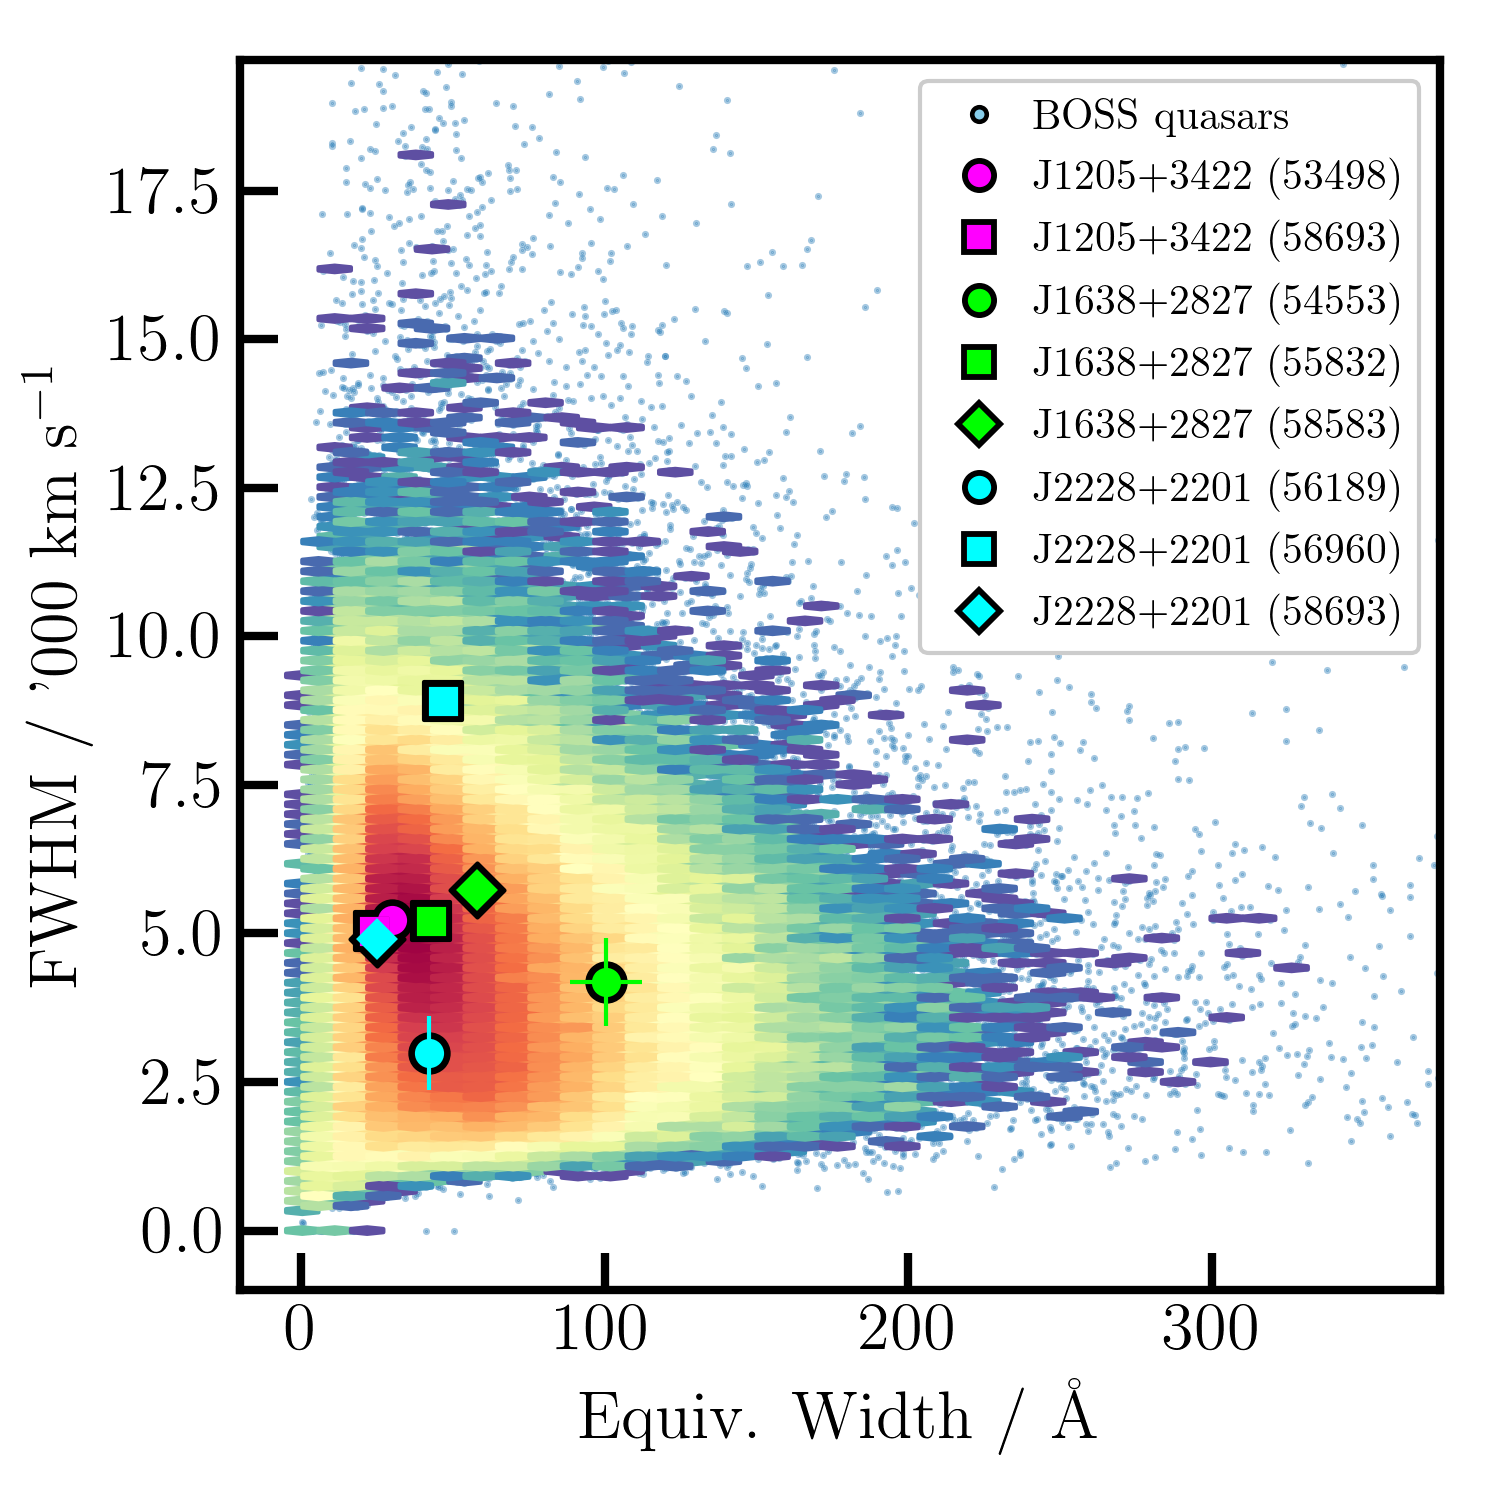
\includegraphics[width=8.5cm, trim=0.2cm 0.2cm 0.0cm 0.2cm, clip]
  {figures/CIV_CLQs_REWvsFWHM_20191029.png}
   \vspace{-12pt}
  \caption[]{The Rest Equivalent Width (REW) vs. Full Width Half Maximum (FWHM) 
of the \civ\ emission line in the BOSS DR12 quasar sample using the catalogue 
of \citet{Hamann2017}. %Note the REW logarithmic scaling.
}
  \label{fig:REWvsFWHM}
\end{figure}
\section{Discussion}
With $t_{\rm dyn} \propto M^{2}$, the variable properties of high-$z$
quasars, generally with more massive SMBHs, has been less well
studied.

%Reasons for this include more massive systems will tend to have longer timescales with e.g. if $t_{\rm dyn} = \sqrt{ R^{3}/GM}$ and $R_{\rm Sch}= 2GM /c^{2}$.
%%
The Balmer series in hydrogen is due to the recombination cascade
between different principal quantum numbers $n$, and
the $n=2$ level \citep[e.g., ][]{Seaton1959a, Seaton1959b}. 
Lower redshift $z<0.9$ CLQs have traditionally been identified via large changes in the
H$\beta$ emission line. H$\beta$ emission is associated with a 2.55 eV energy difference. 
Thus we can place the high-$z$, HIL \civ\ in context of Balmer H$\beta$ CLQs at lower-$z$.

\civ\ is one of the strongest collisionally excited lines in quasar
spectra \citet[e.g.][]{HamannFerland1999}.  The line is most prominent
at n H $\approx$10$10$ cm$-3$ and log $U$$\approx$-1.5, which are the
canonical BELR parameters deduced over from early analysis of the
\civ\ emission \citep{Davidson_Netzer1979}.  A dimensionless
ionization parameter $U\equiv \Phi(H) / c n_{H}$, where $c$ is the
speed of light and $n_{H}$ is the total hydrogen density (H$^{0}$ +
H$^{+}$).

\civ\ probes the photoionization environment produced by the innermost
disk, as indicated by RM time-delay measurements. In standard \citet{SS73}
thin disk models, large changes in the continuum flux are not
permitted over short timescales due to the relatively long viscous
time associated with such disks. Given the observed short timescale
continuum variations, it is not surprising that the \citet{SS73} disk may fail
on other fronts. The \civ\ variations observed in our sources... 
%DO/DO NOT (I can't tell!?! we have to determine this!) fit the Baldwin Effect relationship found by previous authors (cite em again).

%If they DO fit:
This indicates they may comfortably fit into the sample of CIV
variable QSOs explored by \citet{Dyer2019}, and similar to those
authors we suggest slim accretion disk models e.g., 
\citet[][]{Abramowicz1988} or inhomogeneous disk models
\citep[e.g.,][]{DexterAgol2011} may provide viable explanations for
our observations. I want to say a bit more here about the generic
probe of photoionization vs shielding and conditions in the BL region
but that will take more time.

%If they DO NOT fit:
This implies that the variable \civ\ in our sample arises through
different emission mechanisms than is usual for high-$z$ quasar...
%% --and I gotta think more/longer about what else to say here.

\begin{figure}
  \centering
  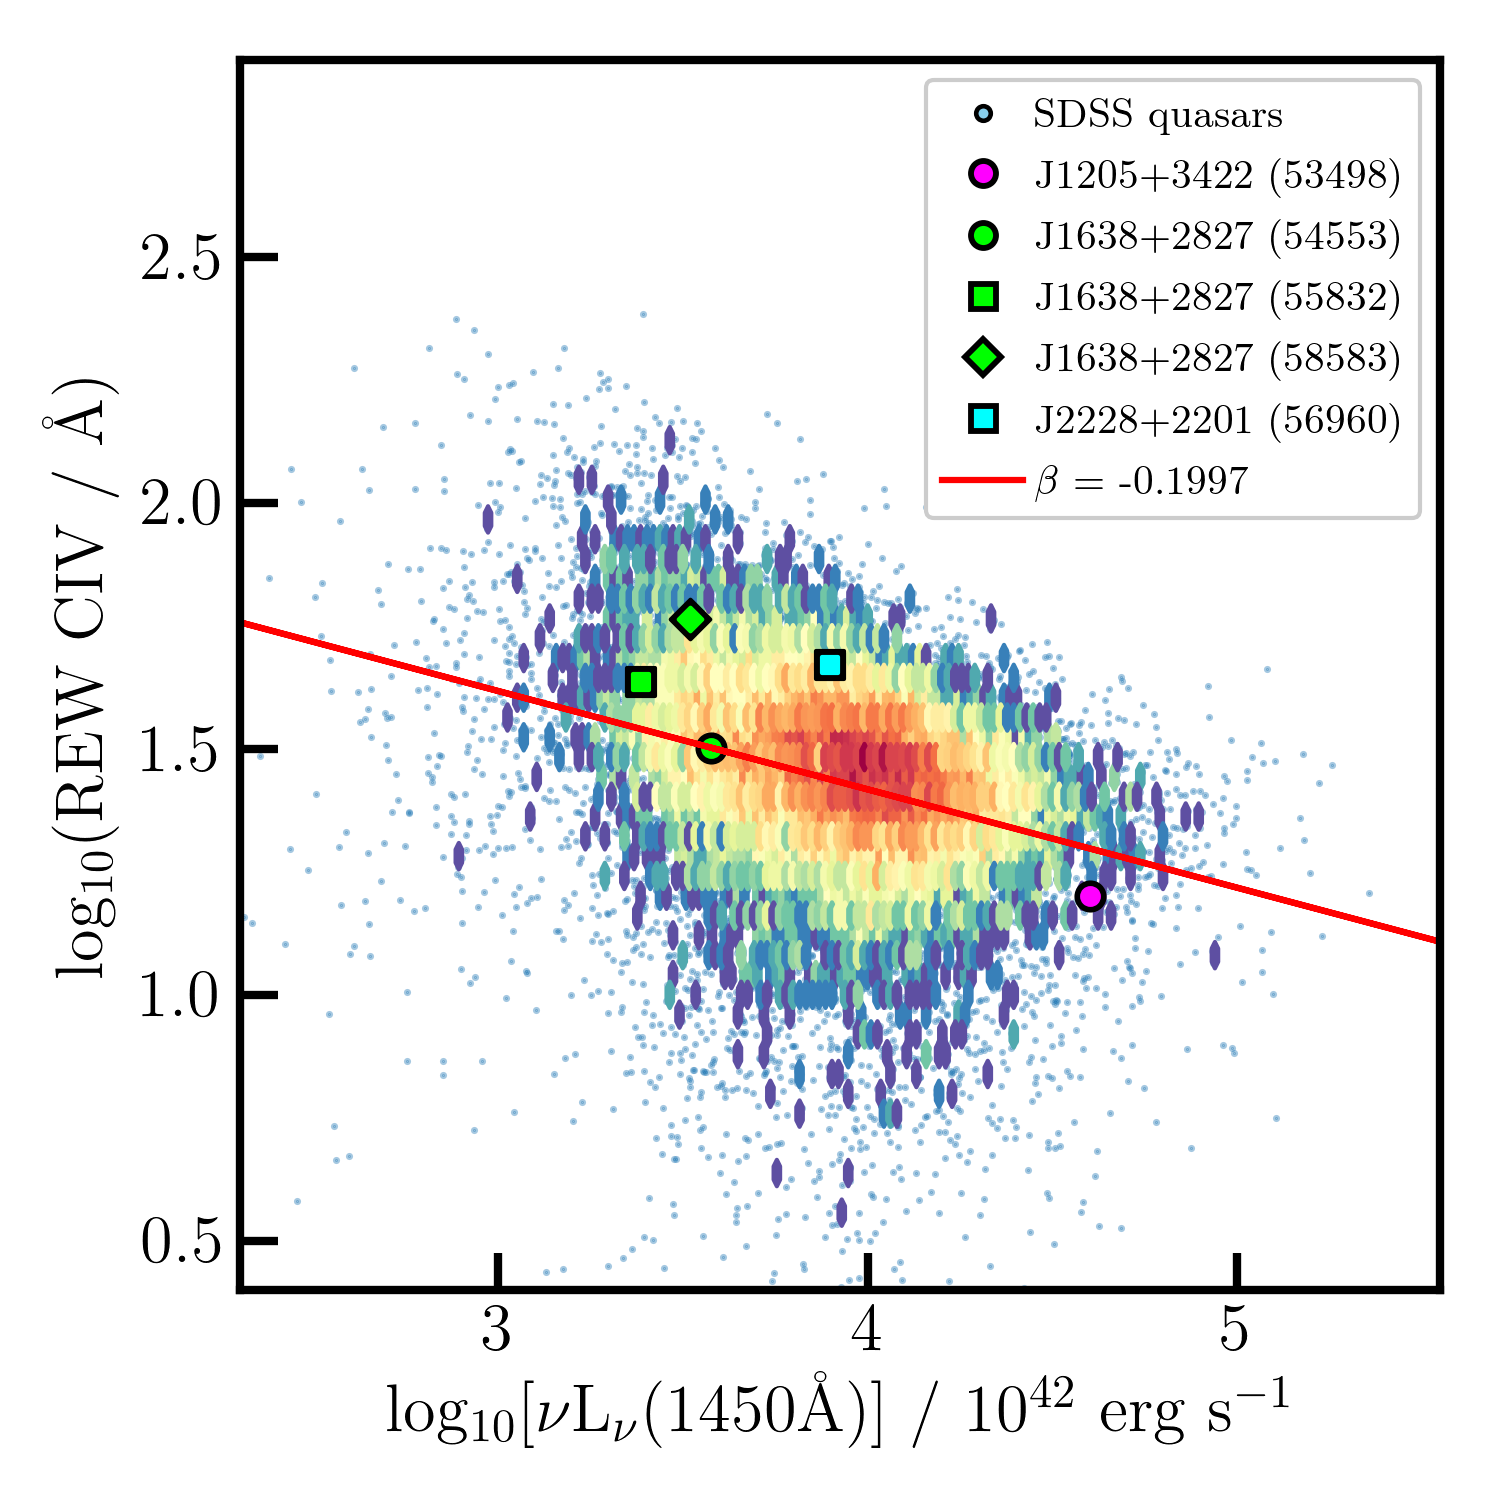
\includegraphics[width=8.5cm, trim=0.2cm 0.2cm 0.0cm 0.2cm, clip]
  {figures/CIV_CLQs_Baldwin_20191108.png}
   \vspace{-12pt}
   \caption[]{The \civ\ Equivalent width and the underlying continuum luminosity,
     commonly referred to as The Baldwin Plot.
     The continuum luminosities are  from \citet{Calderone2017},
     the REW measurements are Table~\ref{tab:Baldwin}.}
  \label{fig:CIV_Baldwin}
\end{figure}
\subsection{The Baldwin Effect}
The variable properties of the rest-frame UV quasar emission lines
have been long studied, with the global (or ensemble) Baldwin Effect
(the anti-correlation between the EW of the emission line and the
underlying continuum luminosity of single-epoch observations of a
large number of AGN, first noted in \citet{Baldwin1977}.  More
recently, the intrinsic Baldwin effect, the same anti-correlation but
in an individual, variable AGN.  

The X-ray Baldwin Effect \citep[e.g., ][]{Iwasawa_Taniguchi1993}... 
\citet{Bachev2004} find a 10-fold decrease in EW \civ\ with Eddington
ratio (decreasing from $\sim$1 to $\sim$0.01), while \nv shows no
change. These trends suggest a luminosity-independent ``Baldwin
effect'' in which the physical driver may be the Eddington ratio.
\citet{Ge2016} Broad emission lines is a prominent property of type I quasi-stellar objects (QSOs). 



\begin{figure*}
  \centering
  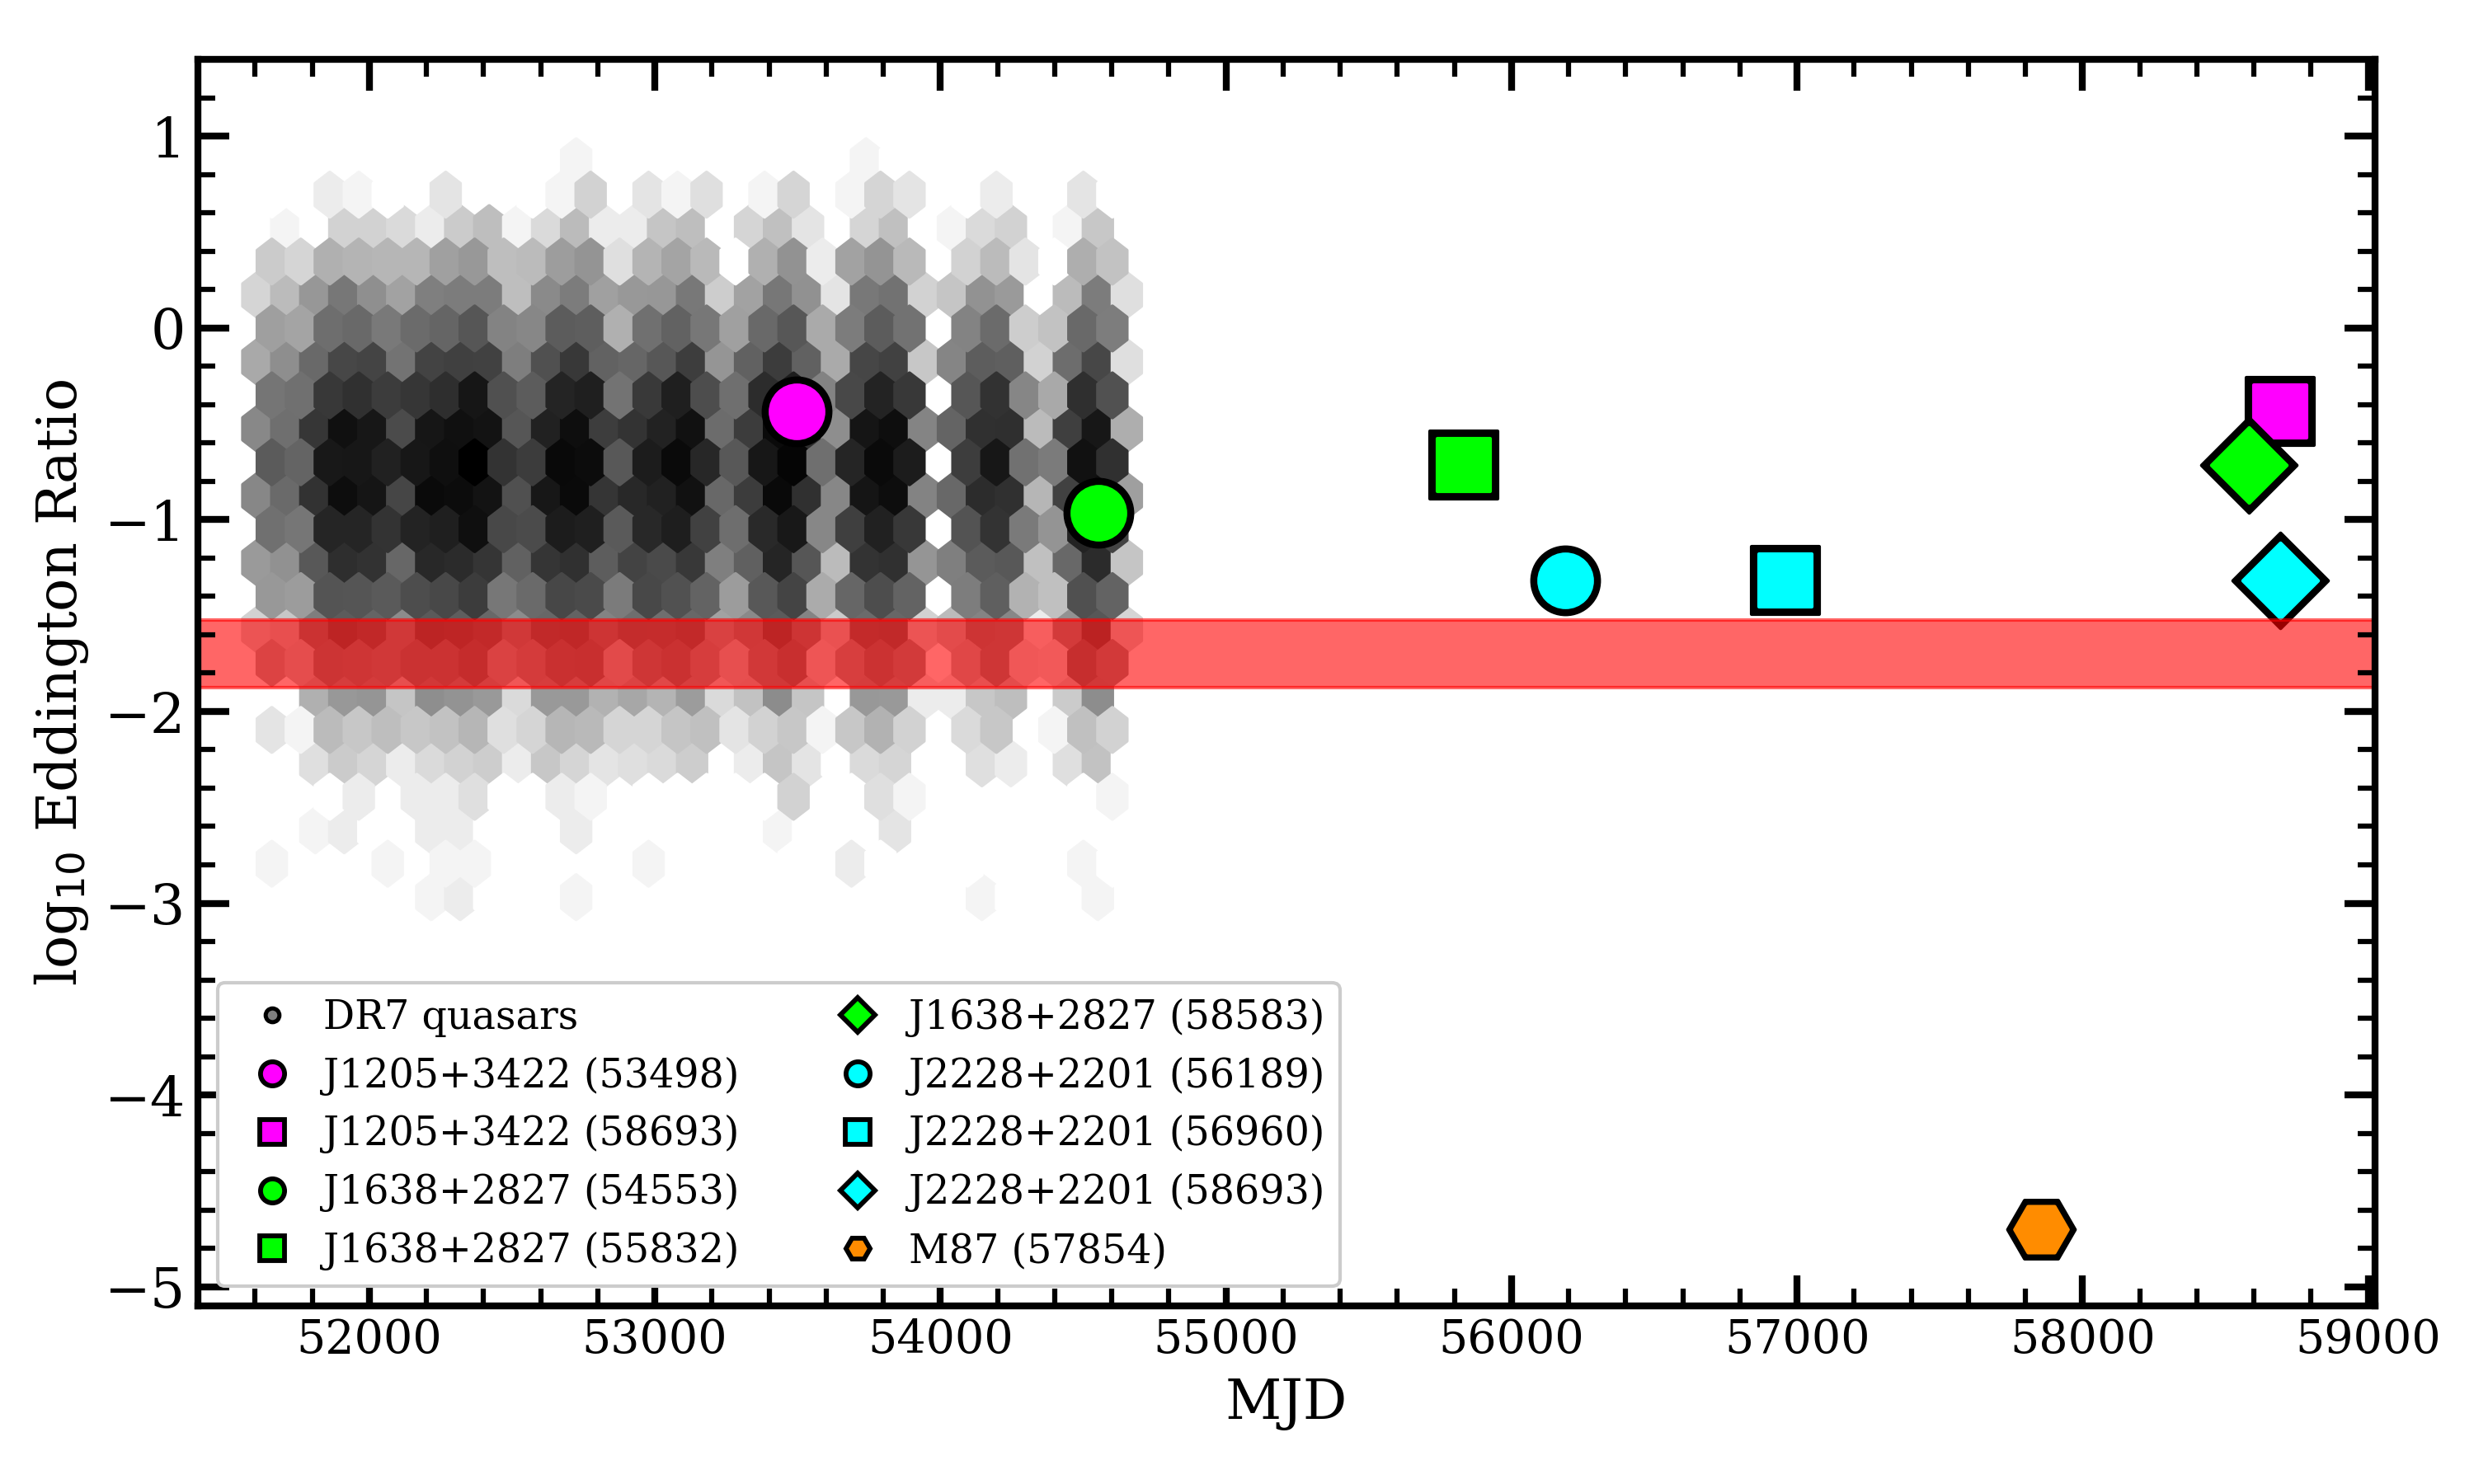
\includegraphics[width=14.5cm, trim=0.2cm 0.2cm 0.0cm 0.2cm, clip]
  {figures/MJD_vs_Eddington_20191104_v0pnt9.png}
  \vspace{-12pt}
  \caption[]{Eddington Ratios of the three \civ\ CLQs and M87.}
  \label{fig:Eddington_ratios}
\end{figure*}
\subsection{Eddington ratios and State Changes} 
The broad UV and optical lines in quasars are most sensitive to the
extreme ultraviolet (EUV) part of the spectral energy distribution
(SED), with \civ\ (and indeed \heii and \nv) being at the higher
energy end of the EUV distribution.

The soft X-ray excess -- the excess of X-rays below 2 keV with respect
to the extrapolation of the hard X-ray spectral continuum model -- is
a very common feature among type 1 active galactic nuclei (AGN). 
\citet{NodaDone2018} note that
The soft X-ray excess produces most of the ionizing photons, so its
dramatic drop leads to the disappearance of the broad-line region,
driving the ``changing-look'' phenomena.  major difference is that
radiation pressure should be much more important in AGNs, so that the
sound speed is much faster than expected from the gas temperature.
%%
This spectral hardening appears similar to the soft-to-hard state
transition in black hole binaries at $L / L_{\rm Edd} \sim 0.02$
(i.e. $\eta_{\rm Edd} \sim -1.7$, where the inner disc evaporates into
an advection dominated accretion flow, while the overall drop in
luminosity appears consistent with the hydrogen ionization disc
instability.  Crucially \citet{NodaDone2018} make the prediction that
all changing-look AGNs are similarly associated with the state
transition at $L / L_{\rm Edd} \sim$a few per cent.
%%
\citet{JiangYF2014, JiangYF2016, JiangYF2019}.
\citet{JiangYF2019arXiv} use global three dimensional radiation
magneto-hydrodynamic simulations to study the properties of inner
regions of accretion disks around a $5 \times 10^{8}$ M$_{\odot}$
black hole with mass accretion rates reaching 7\% and 20\% of the
Eddington value.

We investigate this reporting the Eddington ratios of the three
quasars in Table~\ref{tab:Eddington_ratios}.
%%
Lorem ipsum dolor sit amet, consectetur adipiscing elit. Aliquam porta
sodales est, vel cursus risus porta non. Vivamus vel pretium
velit. Sed fringilla suscipit felis, nec iaculis lacus convallis
ac. Fusce pellentesque condimentum dolor, quis vehicula tortor
hendrerit sed. Class aptent taciti sociosqu ad litora torquent per
conubia nostra, per inceptos himenaeos. Etiam interdum tristique diam
eu blandit. Donec in lacinia libero.

Sed elit massa, eleifend non sodales a, commodo ut felis. Sed id
pretium felis. Vestibulum et turpis vitae quam aliquam convallis. Sed
id ligula eu nulla ultrices tempus. Phasellus mattis erat quis metus
dignissim malesuada. Nulla tincidunt quam volutpat nibh facilisis
euismod. Cras vel auctor neque. Nam quis diam risus.

Nunc semper quam et leo interdum vulputate eu quis magna. Sed nec arcu
at orci egestas convallis. Aenean quam velit, aliquam vitae viverra
in, elementum vel elit. Nunc suscipit aliquet sapien a suscipit. Cras
nulla ipsum, posuere eu fringilla sit amet, dapibus ultricies
nulla. Nullam eu augue id purus mollis dignissim sed et
libero. Phasellus eget justo sed neque pellentesque egestas nec id
arcu. Donec facilisis pulvinar sapien et fringilla. Suspendisse
vestibulum rhoncus sapien id laoreet. Morbi et orci vitae tortor
imperdiet imperdiet. In hac habitasse platea dictumst. Vivamus vel
neque id mi ultrices tristique. Integer quam libero, ornare vel
gravida in, feugiat a ante. Nam dapibus, tellus vitae pellentesque
cursus, dui nisl egestas augue, non fermentum nisl est nec
nisi. Vestibulum nec mi justo, eget dapibus velit.



%%%%%%%%%%%%%%%%%%%%%%%%%%%%%%%%%%%%%%%%%%%%%%%%%%%%%%%%%%%%%%%%%%%%%%%%%%%%%%%%%%%%%%%%%
%%%%%%%%%%%%%%%%%%%%%%%%%%%%%%%%%%%%%%%%%%%%%%%%%%%%%%%%%%%%%%%%%%%%%%%%%%%%%%%%%%%%%%%%%
%%
%%     S E C T I O N     5    S E C T I O N     5    S E C T I O N     5    S E C T I O N     5    S E C T I O N     5    S E C T I O N     5   
%%     S E C T I O N     5    S E C T I O N     5    S E C T I O N     5    S E C T I O N     5    S E C T I O N     5    S E C T I O N     5   
%%     S E C T I O N     5    S E C T I O N     5    S E C T I O N     5    S E C T I O N     5    S E C T I O N     5    S E C T I O N     5   
%%
%%%%%%%%%%%%%%%%%%%%%%%%%%%%%%%%%%%%%%%%%%%%%%%%%%%%%%%%%%%%%%%%%%%%%%%%%%%%%%%%%%%%%%%%%
%%%%%%%%%%%%%%%%%%%%%%%%%%%%%%%%%%%%%%%%%%%%%%%%%%%%%%%%%%%%%%%%%%%%%%%%%%%%%%%%%%%%%%%%%
\section{Conclusions}
In this paper we have reported on three redshift $z>2$ quasars with
dramatic changes in their \civ\ emission lines, the first
`Changing-Look'' quasars at high redshift.  This is also the first
time the changing-look behaviour has been seen in a high-ionization
emission line.

\begin{itemize}
  \item SDSS J1205+3422, J1638+2827 and J2228+2201 show interesting behaviour
in their observed optical light curves, and subsequent spectroscopy
shows significant changes in the \civ\ broad emission line, with both
line collapse and emergence being displayed in rest-frame timescales
of $\sim$240-1640 days.
\item Where observed, the profile of the Ly$\alpha$/\nv emission complex
also changes, and there is tentative evidence for changes in the \mgii
line.
\item Although line measurements from the three quasars show large changes
in the \civ\ line flux-line width plane, the quasars are not seen to
be outliers when considered against the full $z>2$ quasar population
in terms of (rest) Equivalent Width and FWHM properties.
\item 
We put these observations in context with recent ``state-change''
models, but note that even in their `low-state', the \civ\ CLQs are
above $\sim10\%$ in Eddington luminosity.
\end{itemize}

Etiam mollis viverra nisi eget aliquet. Aliquam erat volutpat. Vivamus
tristique, nisl eu malesuada semper, libero tortor convallis elit, a
scelerisque orci nisi lacinia turpis. In lacinia ultrices
volutpat. Proin ultrices luctus tellus, in placerat eros tincidunt
id. Ut varius iaculis quam in consequat. Nulla nec orci est, sit amet
Aliquam ac metus nec odio tempus pharetra sed nec diam. Sed eget arcu
nulla. Etiam elementum ultrices ligula, at iaculis libero feugiat
bibendum. Suspendisse potenti. Nam pharetra adipiscing
euismod. Quisque imperdiet dignissim odio, sed volutpat justo
tincidunt eu. Nunc vehicula pharetra suscipit. Integer aliquet pretium
ipsum vel ultrices. Nam rutrum nibh ac quam pulvinar molestie.



\subsection*{Availability of Data and computer analysis codes} 
All materials, databases, data tables and code are fully available at: 
\href{https://github.com/d80b2t/CIV_CLQs}{\tt https://github.com/d80b2t/CIV\_CLQs}.


\section*{Acknowledgements}
NPR acknowledges support from the STFC and the Ernest Rutherford Fellowship scheme. 
%% KESF \& BM are supported by NSF PAARE AST-1153335. 
%% KESF \& BM thank CalTech/JPL for support during sabbatical.  
\\

\noindent
We thank:
\begin{list}{$\circ$}{}
  \item  Dr. Giorgio Calderone for discussions to the utility of the QSFit routine and line measurements. 
  \item Andy Lawrence, Mike Hawkins and David Homan for useful discussion.
\end{list}

This paper heavily used \href{http://www.star.bris.ac.uk/~mbt/topcat/}{TOPCAT} (v4.4)
\citep[][]{Taylor2005, Taylor2011}.
%%
This research made use of \href{http://www.astropy.org}{\tt Astropy}, 
a community-developed core Python package for Astronomy 
\citep{AstropyCollaboration2013, AstropyCollaboration2018}.

Funding for SDSS-III has been provided by the Alfred P. Sloan
Foundation, the Participating Institutions, the National Science
Foundation, and the U.S. Department of Energy Office of Science. The
SDSS-III web site is
\href{http://www.sdss3.org/}{http://www.sdss3.org/}.
%%
SDSS-III is managed by the Astrophysical Research Consortium for the
Participating Institutions of the SDSS-III Collaboration including the
University of Arizona, the Brazilian Participation Group, Brookhaven
National Laboratory, Carnegie Mellon University, University of
Florida, the French Participation Group, the German Participation
Group, Harvard University, the Instituto de Astrofisica de Canarias,
the Michigan State/Notre Dame/JINA Participation Group, Johns Hopkins
University, Lawrence Berkeley National Laboratory, Max Planck
Institute for Astrophysics, Max Planck Institute for Extraterrestrial
Physics, New Mexico State University, New York University, Ohio State
University, Pennsylvania State University, University of Portsmouth,
Princeton University, the Spanish Participation Group, University of
Tokyo, University of Utah, Vanderbilt University, University of
Virginia, University of Washington, and Yale University.

This publication makes use of data products from the Wide-field
Infrared Survey Explorer, which is a joint project of the University
of California, Los Angeles, and the Jet Propulsion
Laboratory/California Institute of Technology, and NEOWISE, which is a
project of the Jet Propulsion Laboratory/California Institute of
Technology. WISE and NEOWISE are funded by the National Aeronautics
and Space Administration. No animals were harmed in the production of
this paper, but there was a large spider in NPRs apartment that
``vanished''.

\bibliographystyle{mnras}
\bibliography{tester_mnras}


% Don't change these lines
\bsp	% typesetting comment
\label{lastpage}
\end{document}


\end{document}